%%%%%%%%%%%%%%%%%%%%%%%%%%%%%%%%%%%%
%%  Autho: 	Tekoh Palma Achu
%%  Department: 	Computer Science
%%  Faculty: 	Faculty of Computer Science
%%  University: University of Yaounde I
%%  Academic Year: 	2022-2023
%%%%%%%%%%%%%%%%%%%%%%%%%%%%%%%%%%%%



\documentclass[11pt,aspectratio=169]{beamer}
%preamble section
%%%%%%%%%%%%%
%THEME & TEMPELATE
%%%%%%%%%%%%%
\usetheme[compress]{Dresden}
\usecolortheme{beetle}
\newcommand*\oldmacro{}%
\let\oldmacro\insertshorttitle%
\renewcommand*\insertshorttitle{%
	\oldmacro \hspace{0pt plus 1 filll}{\raggedright\insertframenumber\,/\,\inserttotalframenumber}}

\setbeamercolor{normal text}{fg=black,bg=white}
\setbeamercolor*{palette sidebar primary}{fg=black}
\setbeamercolor{structure}{fg=black}
\setbeamercolor{block title}{bg=beetle@other,fg=white}
\setbeamercolor{block body}{bg=white,fg=black}
\setbeamertemplate{blocks}[rounded][shadow=true]
\setbeamertemplate{navigation symbols}{}
\setbeamercolor{title}{bg=blue!55!black, fg=white}
\setbeamercolor{frametitle}{fg=beetle@other}
\setbeamertemplate{title page}[default][colsep=-4bp,rounded=true]
\setlength{\parskip}{0.5pt}



%%%%%%%%%%%%%
%Importing Packages
%%%%%%%%%%%%%
\usepackage{graphicx}
\usepackage{colortbl}


\begin{document}

	

	
	\title[A Novel Approach to Mobile Money Fraud Detection and Prediction using DLSH]{A Novel Approach to Mobile Money Fraud Detection and Prediction Using Dynamic Locality Sensitive Hashing(DLSH)}
	
	
	
	\author[Tekoh Palma Achu $|$ 19W2615] % (optional, for multiple authors)
	{ {A presentation by :} \vspace{0.1cm }  \\  \textbf{TEKOH PALMA ACHU} \\ Registration Number: 19W2615 \\ \vspace{0.25cm }
		 Under the supervision of : \vspace{0.1cm }\\ \textbf{Dr. DJAM Xaveria Youh KIMBI  } \\ Senior Lecturer , UYI}
	
	\institute[University of Yaounde I]{University of Yaounde I \\ \tiny{Department of Computer science}}	
	
	\date{\today}
	%%Coverpage Section
	%\section{Intro}
	{
		\setbeamertemplate{headline}{}
	\begin{frame}[plain]
		%\titlepage
		\maketitle
	\end{frame}
}

	\section{Roadmap}
	\begin{frame}{\centering \raisebox{-1.9pt}{
\includegraphics[width=0.5cm]{./assets/map.png}} Presentation Roadmap  }
		%somecontent here
		\begin{block}{\centering  Presentation Plan }
			\begin{itemize}
				\item Context
				\item Problem Statement
				\item Aim and Objectives
				\item Research Question
				\item Review of state of the art
				\item Research Methodology
				\item Results and Discussion
				\item Conclusion
				
			\end{itemize}
		\end{block}
	\end{frame}


	\section{Context}
		\begin{frame}
			%somecontent here
			 \begin{center}
			 	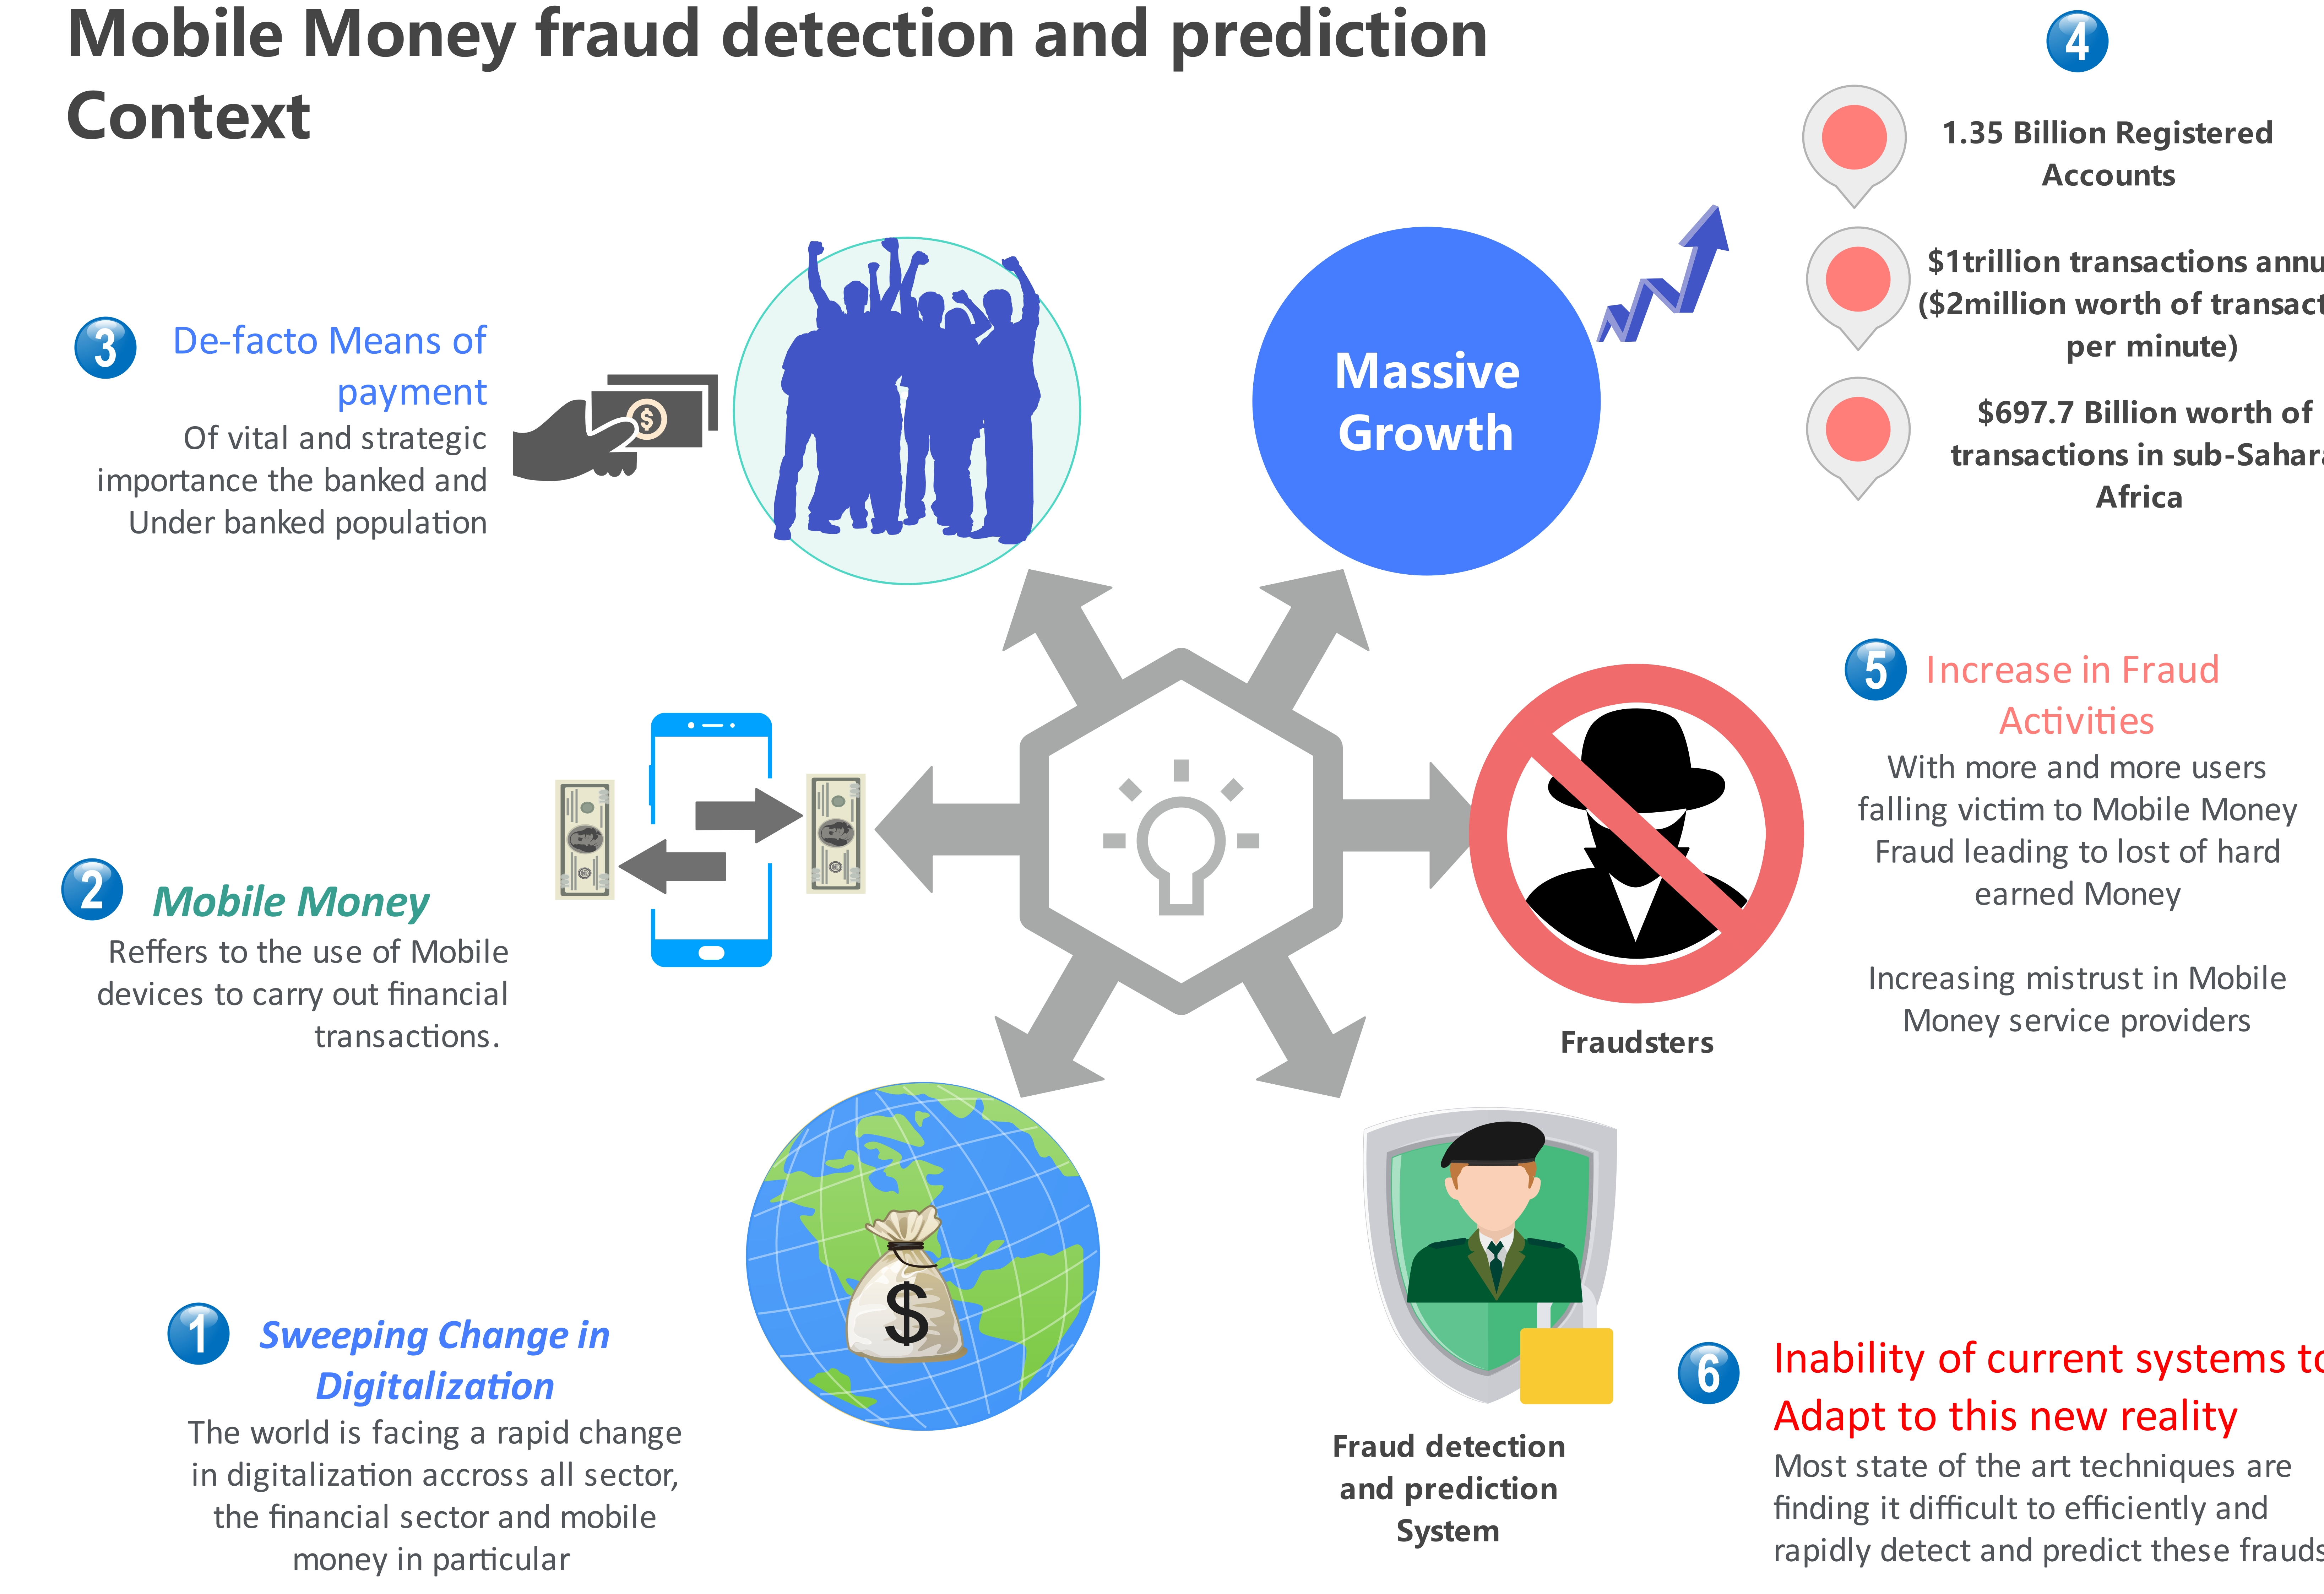
\includegraphics[width=\textwidth,height=183pt]{assets/context.jpg}
			 \end{center}
	
		\end{frame}

	\section{Problem Statement}
		\subsection{Problems faced by Mobile Money Users}
		
			\begin{frame}{Problem Statement}
			%somecontent here
			\begin{block}{Problems faced by Mobile Money Users}
					\begin{itemize}
						\item More and More fraudsters use Smishing mobile Money Messages to trick users to perform fraudulent transactions or reveal Pin code
						\item Users loose their phones which ends up in the hands of fraudsters who end up effectuating fraudulent transactions
					\end{itemize}
			\end{block}			
		\end{frame}	
	
		\subsection{Problems related to State of the art Mobile Money Fraud Detection and Prediction systems}
		\begin{frame}{Problems Statement}
			%somecontent here
			\begin{block}{Problems related to state of the art  Mobile Money fraud Detection and Prediction}
					\small {		
					\begin{itemize}
						\item use arbitrary threshold assignment mechanism to combat mobile money fraud which is highly inefficient.
						
						\item Are not Flexible and very costly to maintain and update[6]
						
						\item Are black boxes that are difficult to trace the rationale used for detection and prediction [7]
						
						\item Are Very expensive to build and don’t scale well on massive amounts of dataset[8]
						
						\item Do a trade-off between efficiency and speed and don’t perform high on both measures.
						
					\end{itemize}
			}
			\end{block}
		\end{frame}	
	
		\subsection{\tiny{Illustrative Example: Mobile Money fraud detection and prediction Problem}}
		\begin{frame}{\normalsize{{\textbf{Illustrative Example:} Mobile Money fraud detection and prediction Problem}}}
			%somecontent here
			%\begin{block}{The Mobile Money fraud Detection and Prediction Illustrative example}
			\small
			\textbf{Let:}\\ 
			- $U$ represent a set of \textbf{$m$} Mobile Money users for a given service provider \centering  $U=\{u_1,u_2,\cdots,u_m \}$\\
			
			-The communication $C_{STMR}$ between $u_x, u_y \in U$ be modeled as follows:
			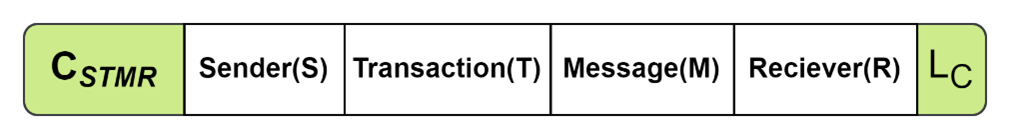
\includegraphics[width=0.5\textwidth]{./assets/model.png}
			
				\begin{columns}
					\column{0.5\textwidth}
				\textbf{Where:}\\
				\footnotesize{
				\begin{enumerate}[-]
					\item $C_i$ is the $i^{th}$ communication
					\item $S =$ Sender or initiator of $C_{STMR}$ with attributes $\{s_i^1,s_i^2,\cdots,s_i^p \}$\\
					\item  $T = $ Mobile Money Transaction  with attributes $\{T_i^1,T_i^2,\cdots,T_i^u \}$\\
					\item $M = $ Mobile Money Message  with attributes $\{M_i^1,M_i^2,\cdots,M_i^v \}$\\
				\end{enumerate}
				 
				}
						
						
				
					\column{0.5\textwidth}
					\footnotesize{
					\begin{enumerate}[-]
					\item $R = $ Receiver or Receptor of $C_{STMR}$ with attributes $\{R_i^1,R_i^2,\cdots,R_i^q \}$\\
					\item $L_c = $ label for $C_{STMR}$ ie Fraudulent or Non-Fraudulent\\
					\item With $S,R \in U$
				\end{enumerate}
			}
	
				\end{columns}
				
			%\end{block}
			
						
		\end{frame}	
	
			\subsection{Illustrative Example Continued}
		\begin{frame}{\normalsize{{\textbf{Illustrative Example:} Mobile Money Communication tree}}}
		%somecontent here
		%\begin{block}{The Mobile Money fraud Detection and Prediction Illustrative example}

			
			\centering
			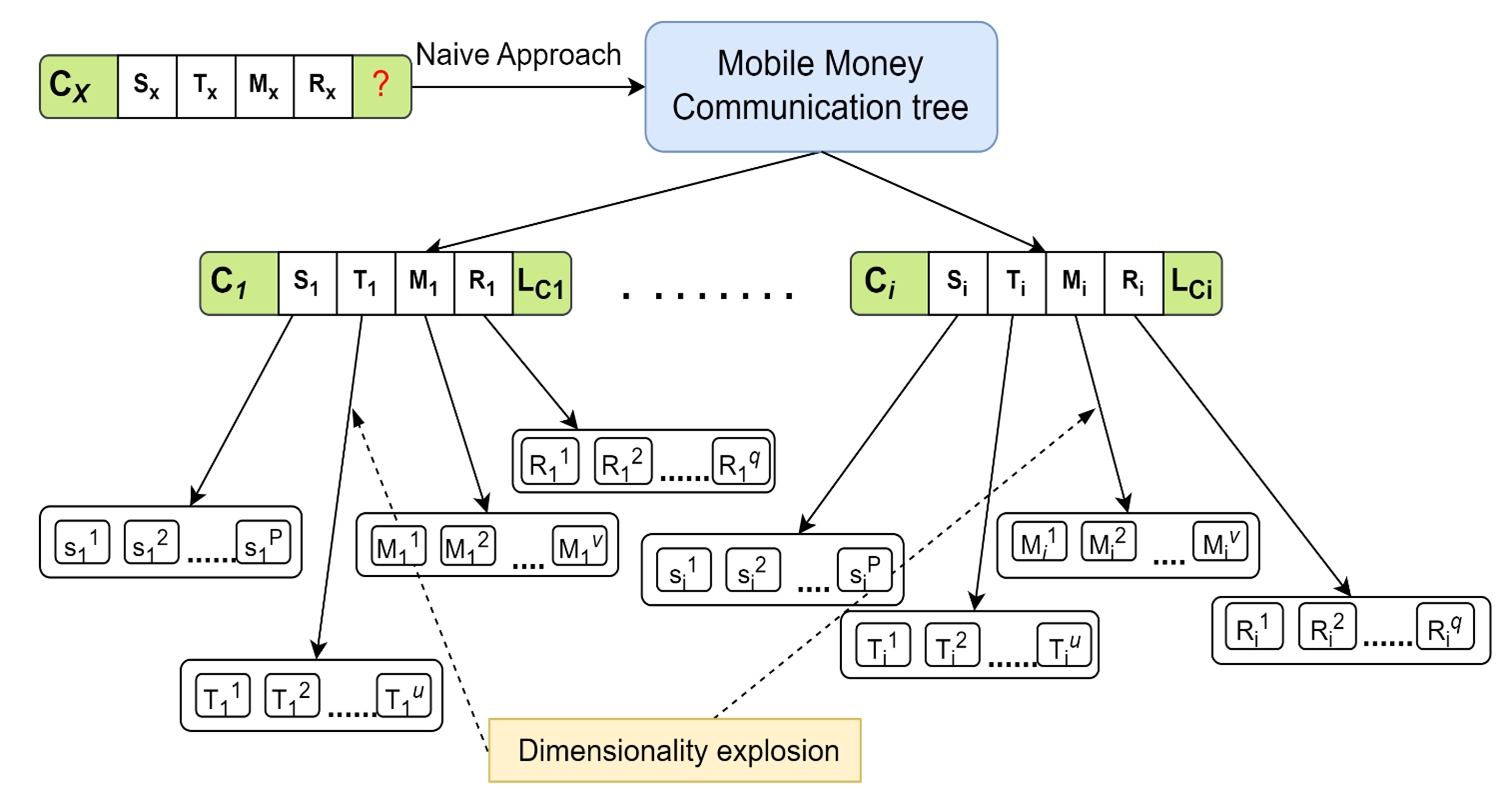
\includegraphics[width=250pt]{./assets/example.png}
			\underline {Dimensionality Explosion in Mobile Money Communication Tree}
			\
	
		
		%\end{block}
		
		
		
	\end{frame}	

	\begin{frame}
		\small{
			Given a communication tree of 100,000 communications(search space representation)\\
			\textbf{Questions}\\
			\begin{itemize}
				\item How efficiently can we Identify similar transactions in our search space?
				\item How fast can we do the identification process? 
			\end{itemize}
		
		\textbf{Answers}\\
			\begin{itemize}
				\item Need to perform exhaustive search throughout the entire search space to guarantee efficiency
				
				\item Perform fast pair-wise comparison of communication instance with inference communications 
		
			\end{itemize}
		\textbf{At what Cost?}\\
		Number of pair-wise Comparison $= \frac{100,000 \times 99,999}{2}\simeq 5,000,000,000$ operations\\
		\underline{Standard PC:}
		\begin{columns}
			\column{0.5\textwidth}
			\begin{itemize}
				\item Performs 10,000 operations per second
				\item $\simeq \alert{5.787days}$ to perform computation 
			\end{itemize}
		\column{0.5\textwidth}
		\begin{itemize}
			\item For a dataset of 5-dimensions like $C_{STMR}$ it takes \alert{28.9 days} 
			
		\end{itemize}
		\end{columns}
		
	}
		%\end{block}
		
		
		
	\end{frame}	
	
		\section{Aim and Objective}
			\begin{frame}{ Aim and Objective}
				%somecontent here
				
				\begin{block}{Aim}
					The aim of this research work is to use dynamic locality sensitive hashing to  efficiently and rapidly detect and predict mobile money fraud related to SMS and Mobile Money transactions.
				\end{block}
		
				\begin{block}{Objectives}
					\begin{itemize}
						\item Use  dynamic locality sensitive hashing techniques to efficiently and rapidly detect and predict mobile money SMS fraud.
						
						\item Use dynamic Locality sensitive hashing technique to efficiently and rapidly detect and predict mobile money transaction fraud
						
					\end{itemize}
				\end{block}
				
				
				
			\end{frame}
		
		
	\section{Research Question}
		\begin{frame}{\centering Research Question}
			%somecontent here
			\begin{block}{Main Research Question}
				\textbf{RQ:} How can a novel dynamic locality sensitive hashing approach be used to efficiently and rapidly detect and predict mobile money fraud related to SMS and transactions?
				
			\end{block}
			
			\begin{block}{Sub Research Questions}
				\begin{itemize}
					\item \textbf{RQ1:}  How can we use a novel dynamic locality sensitive hashing techniques to efficiently and rapidly detect and predict mobile money SMS fraud? 
					
					
					\item \textbf{RQ2:}  How can a novel dynamic Locality sensitive hashing technique to efficiently and rapidly detect and predict mobile money fraud related to transactions? 
					
					
				\end{itemize}
			\end{block}
		\end{frame}
		


		
	\section{Review of State of the art}
	\begin{frame}{Review of State of the art Mobile Money Prediction and detection Systems}
		\begin{table}
			\begin{center}
				{\tiny
					%\begin{tabular}{|>{\columncolor{green}}c|c|c|c|c|c|}
					\begin{tabular}{ | m{2.5 cm} | m{2.5 cm} | m{4 cm} | m{4 cm} |}  
						\hline
						\rowcolor{orange}
						Approach and Author & Problematic & Methodology & Limitations  \\
						\hline
						
						\textbf{Mobile Money SMS Fraud Detection: Josh et al [2021]}
						& Detection of Fraud in Mobile Money SMS
						& Application of SVM, logistic regression, Multinomial naive bayes
						classifier, Random Forest and CNN while focusing on different feature extraction
						techniques (TF-IDF, count vectorizer, Tokenizer, Transformer) and their impact on the
						performance of machine learning model
						& 
						- Fail to address Mobile Money transaction Fraud \newline
						- Did not use state-of-the-art Semantic encoding scheme such as Google USE. \newline
						- Computationally costly to train models\newline \\
						\hline
						
						\textbf{Efficiency of SVM, GBDT and Naive Bayes algorithms in Mobile Money Transaction fraud detection: Botchey et al [2020]}
						& 
						Determining the efficiency of SVM, GBDT and Naive Bayes algorithms in Mobile Money Transaction fraud detection
						& 
						Apply two (2) under sampling (RandomUnderSampler, NearMiss)
						and two (2) oversampling (RandomOverSampler, SMOTE) technique and finally a
						hybrid of both sampling techniques on the imbalance dataset Evaluate the performance
						of SVM, GBDT and Na¨ıve Bayes algorithms in MMT fraud detection while evaluating
						the impact of Sampling techniques on the imbalance data-set.
						& 
						- Does Not address SMS fraud \newline
					 	-  Model serves as a black box \newline
						- Data intensive and very costly to train \\
						\hline
						
						\textbf{Improved Case based reasoning(CBR): Adedoyin et al [2017]}
						&Identification of Mobile Transfer fraud in Mobile Money Environment. &Improved CBR approach by combining features to single dimension
						vector then using Genetic algorithm to compute optimal feature weights then using
						KNN for classification of MMT into normal or fraudulentt & - computationally very expensive and does not scale well on massive amounts of
						data. \newline
						- Dataset used to evaluate this approach was very small(2000)  \\
						\hline		
					\end{tabular}
				}
			\end{center}
			\caption{Review of State of the Art Technique}
			\label{table 1}
		\end{table}
	\end{frame}




		\subsection{Mobile Money SMS Fraud detection Josh [2021]}
		\begin{frame}{\small{\textbf{\raisebox{-1.9pt}{
\includegraphics[width=0.5cm]{./assets/note.png}} Review of State of the Art Technique}}}
			%somecontent here
			\begin{block}{Mobile Money SMS Fraud Detection: Josh et al [2021]}
				\textbf{Problematic:} 
					Detection of Fraud in Mobile Money SMS\\
				
				\textbf{Methodology:} 
				Application of SVM, logistic regression, Multinomial naive bayes classifier, Random Forest and CNN while focusing on different feature extraction techniques (TF-IDF, count vectorizer, Tokenizer, Transformer) and their impact on the performance of machine learning model
			
			\end{block}
		
			
					\begin{block}{ Limitations}
						\begin{itemize}
							\item Fail to address Mobile Money transaction Fraud
							\item Did not use state-of-the-art Semantic encoding scheme such as Google USE.
							\item Computationally costly to train models
						\end{itemize}
					\end{block}
			
			
		\end{frame}
	
	\subsection{ Determining the efficiency of SVM, GBDT and Naïve Bayes algorithms in MMT fraud detection. Botchey et al [2020]}
	\begin{frame}
		%somecontent here
		\begin{block}{Efficiency of SVM, GBDT and Naïve Bayes algorithms in Mobile Money Transaction fraud detection. Botchey et al [2020]}
			\textbf{Problematic:} 
			Determining the efficiency of SVM, GBDT and Naïve Bayes algorithms in Mobile Money Transaction fraud detection
			
			\textbf{Methodology:} 
			-  Apply two (2) under sampling (RandomUnderSampler, NearMiss) and two (2) oversampling (RandomOverSampler, SMOTE) technique and finally a hybrid of both sampling techniques on the imbalance dataset
			Evaluate the performance of SVM, GBDT  and Naïve Bayes algorithms in MMT fraud detection while evaluating the impact of Sampling techniques on the imbalance data-set.
			
		\end{block}
			\begin{block}{Limitations}
				\begin{itemize}
					\small
					\item Does Not address  SMS fraud
					\item Model serves as a black box
					\item Data intensive and very costly to train
				
				\end{itemize}
			\end{block}
		
	
	\end{frame}


\subsection{Improved Case based reasoning(CBR)}
	\begin{frame}{\small{\textbf{\raisebox{-1.9pt}{
\includegraphics[width=0.5cm]{./assets/note.png}} Review of State of the Art Technique}}}
		%somecontent here
		\begin{block}{Improved Case based reasoning(CBR): Adedoyin et al [2017]}
			\textbf{Problematic:} 
			Identification of Mobile Transfer fraud in Mobile Money Environment.\\
			
			\textbf{Methodology:} 
			Improved CBR approach by combining features to single dimension vector then using Genetic algorithm to compute optimal feature weights then using KNN for classification of MMT into normal or fraudulent
			
			
		\end{block}
		
			\begin{block}{ Limitations}
				\begin{itemize}
					\item computationally very expensive and does not scale well on massive amounts of data
					\item Dataset used to evaluate this approach was very small(2000)
				
				\end{itemize}
			\end{block}
	
		
	\end{frame}
	
	
	\section{Research Method}
		\subsection{Overview of Methodology}
		\begin{frame}{\raisebox{-1.9pt}{
\includegraphics[width=0.5cm]{./assets/idea.png}} Overview of Our Methodology(DLSH)}
			%somecontent here
			\begin{center}
				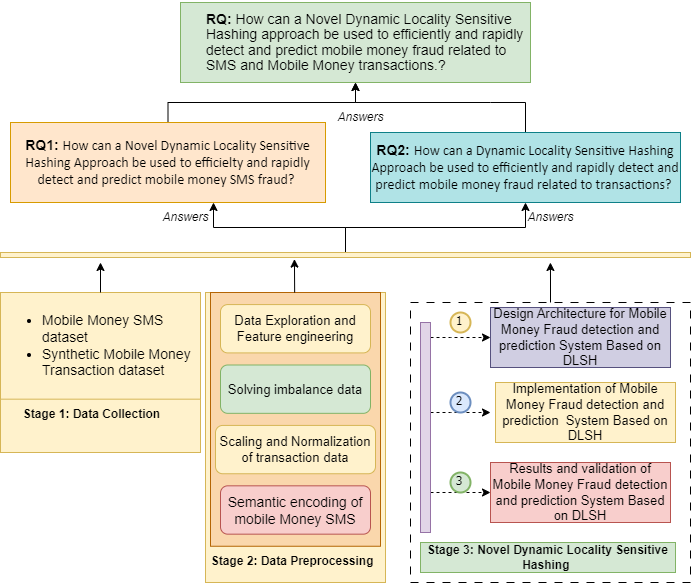
\includegraphics[width=325pt,height=180pt]{assets/methodology.png}
			\end{center}
		
		\end{frame}
	
	\subsection{Stage-1: Data Collection}
		\begin{frame}{\raisebox{-1.9pt}{
\includegraphics[width=0.5cm]{./assets/idea.png}} Stage-1: Data Collection}
			%somecontent here
			\begin{block}{Collection of Mobile Money Transaction datatset}
				\begin{enumerate}
					\item Synthetic data from Paysim simulator as proposed by Lopez et al $[3]$. 
					\item Data was generated using a real-world data obtained from a mobile money operator operating in over 14 African countries. 
				\end{enumerate}
			\end{block}
		
			\begin{block}{Collection of Mobile Money SMS datatset}
				\begin{enumerate}
					\item Spam collection dataset Tiago et al $[29]$   
					\item 100 Mobile Money Spam SMS gotten from colleagues, friends and family.
				\end{enumerate}
			\end{block}

		\end{frame}
	
		\subsection{Stage-2: Data Preprocessing}
	\begin{frame}{\raisebox{-1.9pt}{
\includegraphics[width=0.5cm]{./assets/idea.png}}  Stage-2: Data Preprocessing}
		%somecontent here
		\begin{block}{Preprocessing of Mobile Money Transaction datatset}
			\begin{enumerate}
				\item \textbf{Data exploration:} To gain better understanding of data representation and elimination of data anomalies and null values. 
				 \item \textbf{Feature Engineering:} Sklearn’s ExtraTreesClassifier feature importance measure and Chi Square score to eliminate features that don't contribute to prediction
				 \item \textbf{Balancing of Data(SMOTE-Tomek):} Applied SMOTE to increase minority class and Tomek to eliminate noise introduced by SMOTE
			\item \textbf{Min-Max Normalization:} to reduce the range of data points and hence speed up training and testing phase
			\end{enumerate}
		\end{block}
		
	\end{frame}

	\begin{frame}{\raisebox{-1.9pt}{
\includegraphics[width=0.5cm]{./assets/idea.png}} Stage-2: Data Preprocessing}
		%somecontent here
		\begin{block}{\small Preprocessing of Mobile Money SMS datatset}
			\begin{enumerate}
				\item \textbf{Data exploration:} To gain better understanding of data representation and elimination of data anomalies and null values. 
				\item \textbf{Semantic Encoding:} To capture and represent the Semantic meaning of Mobile Money messages in form that a computer can understand we used Google USE(Universal Sentence Encoder).
			\end{enumerate}
		\end{block}
	\end{frame}
	
	
	
		\subsection{Stage-3: Dynamic Locality Sensitive Hashing (DLSH)-Training Phase}
		\begin{frame}{\raisebox{-0.6pt}{
\includegraphics[width=0.5cm]{./assets/idea.png}}\small Stage 3: Dyanamic Locality Sensitive Hashing (DLSH) -Training Architecture}
		
			%somecontent here
			\begin{center}
				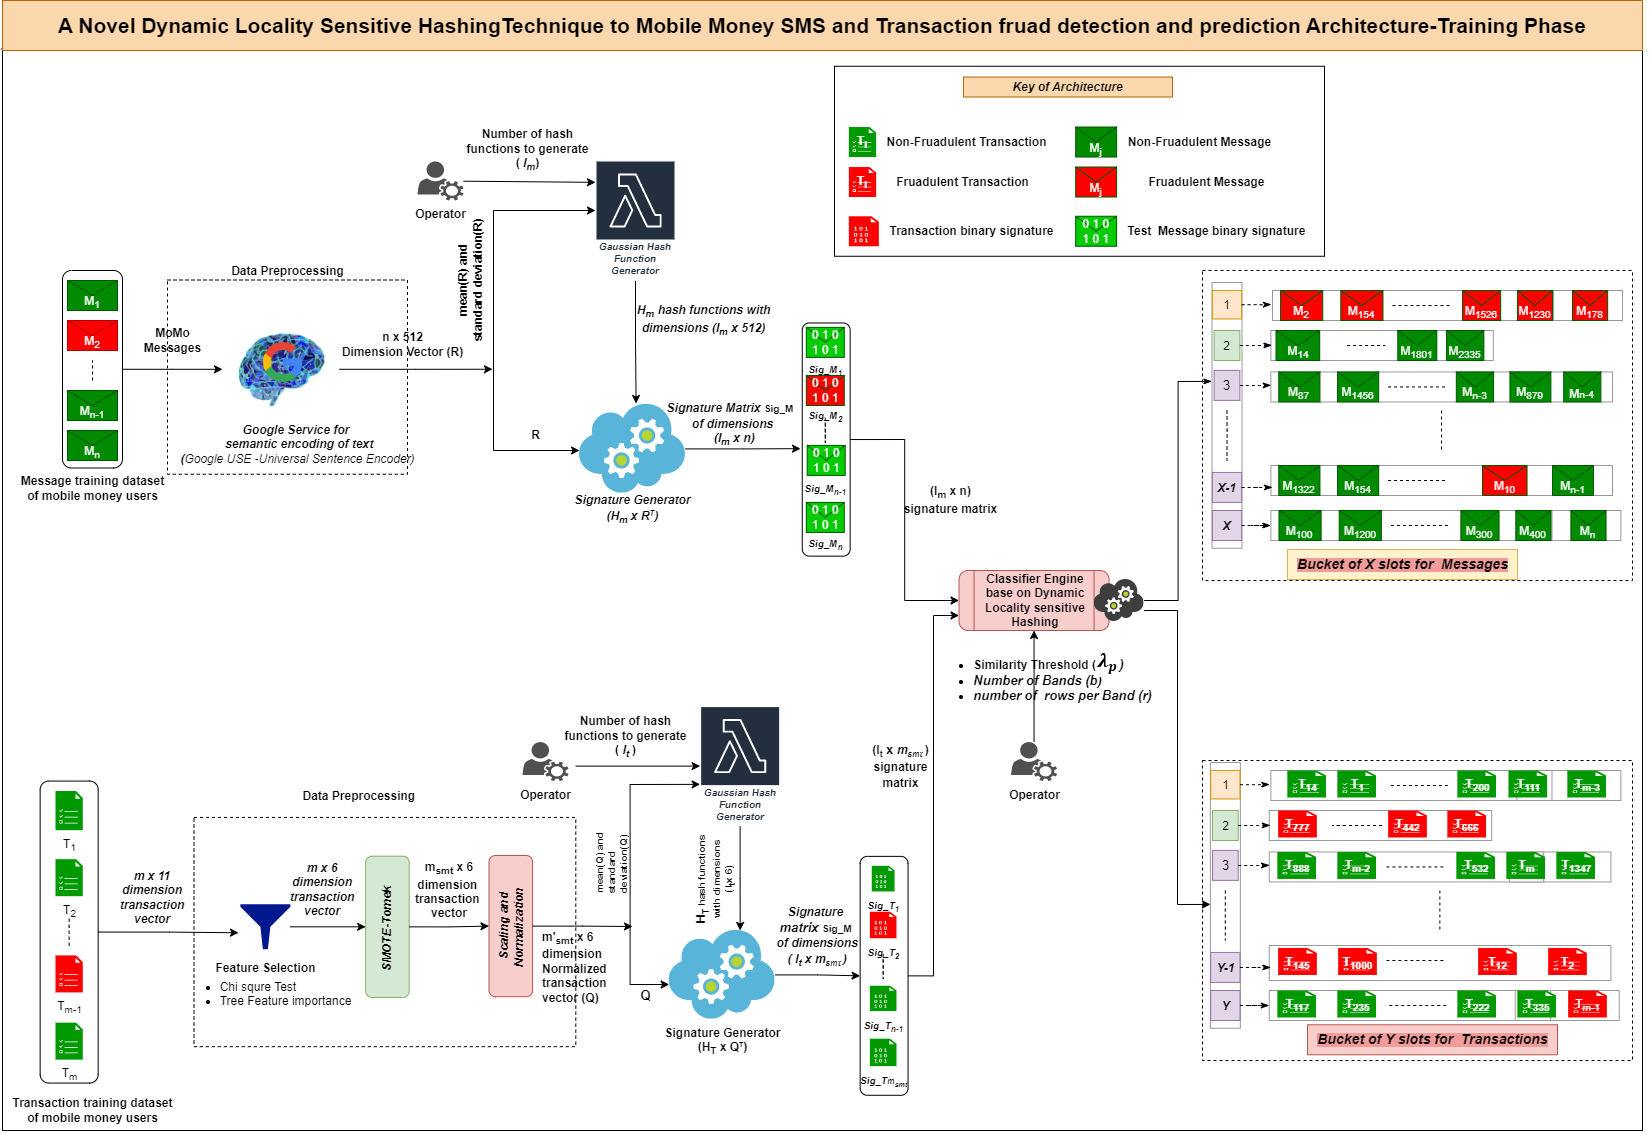
\includegraphics[width=\textwidth,height=183pt]{assets/training1.png}
			\end{center}
			
		\end{frame}
	
			\subsection{Stage-3: Dynamic Locality Sensitive Hashing (DLSH)-Testing Phase}
		\begin{frame}{\raisebox{-1.9pt}{
\includegraphics[width=0.5cm]{./assets/idea.png}} \small Stage 3: Dyanamic Locality Sensitive Hashing (DLSH) -Testing Architecture}
			%somecontent here
			\begin{center}
				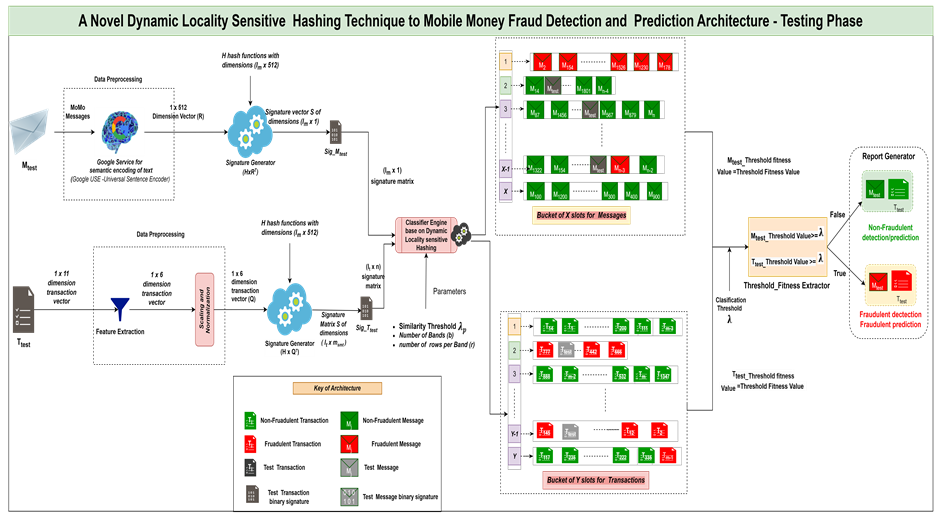
\includegraphics[width=\textwidth,height=169pt]{assets/testing.png}
			\end{center}
			
		\end{frame}
	
	\begin{frame}{\raisebox{-1.9pt}{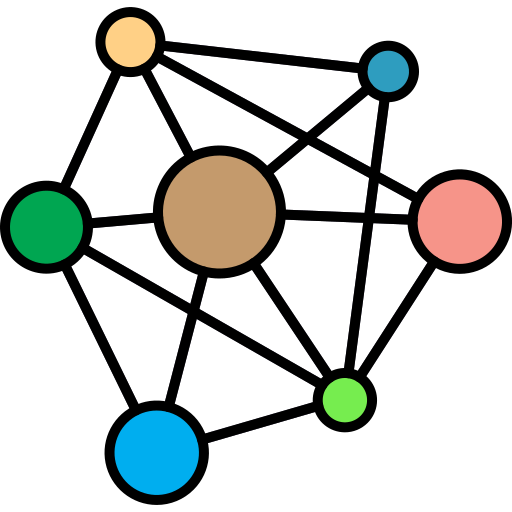
\includegraphics[width=0.5cm]{./assets/algorithm.png}} \small Dynamic Locality Sensitive Hashing (DLSH) Algorithms}
		\begin{columns}
			\column{0.5\textwidth}
			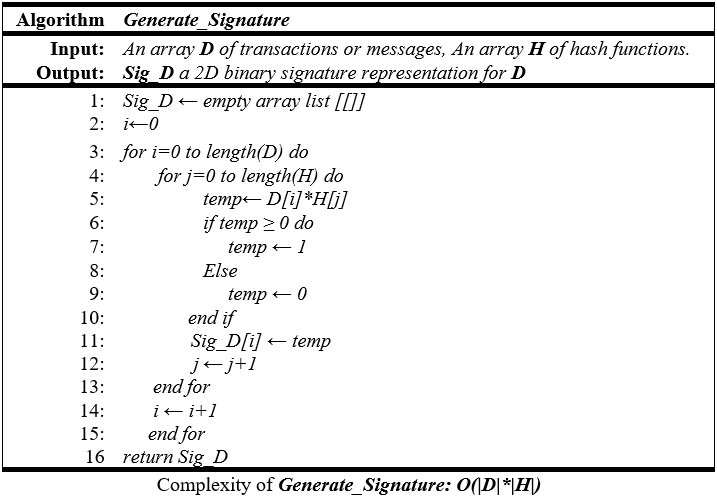
\includegraphics[width=\textwidth,height=169pt]{assets/Signature.png}
			
			\column{0.5\textwidth}
			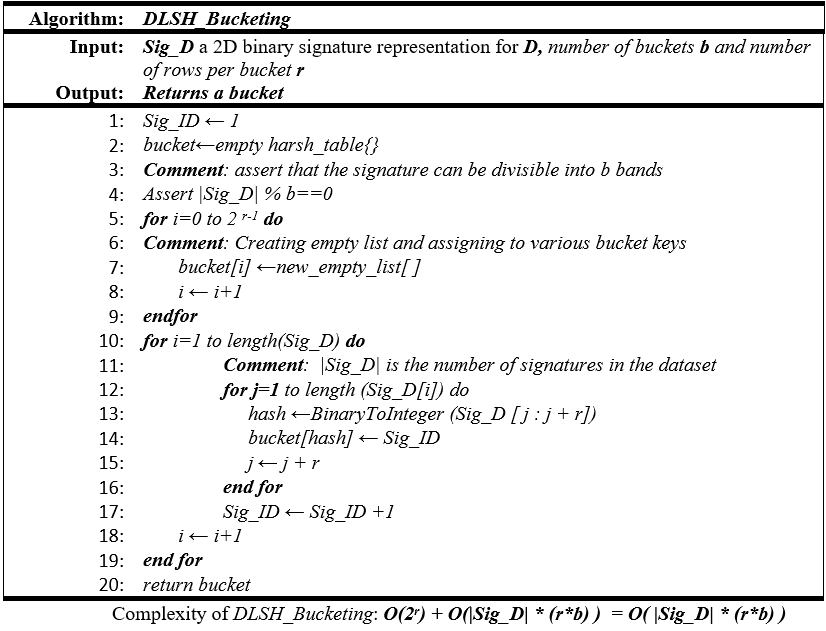
\includegraphics[width=\textwidth,height=175pt]{assets/bucketing.png}
	\end{columns}
	\end{frame}

	\begin{frame}{\raisebox{-1.9pt}{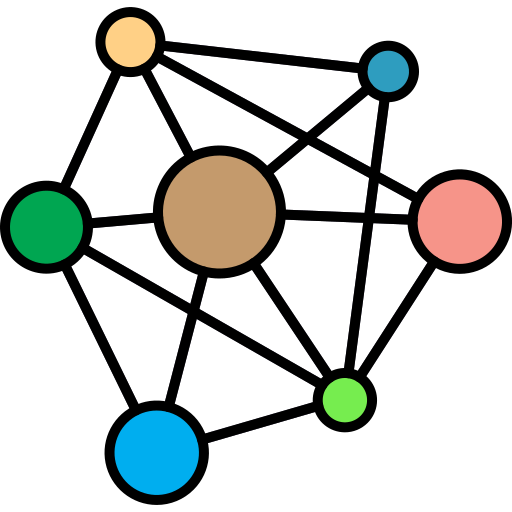
\includegraphics[width=0.5cm]{./assets/algorithm.png}} \small Dynamic Locality Sensitive Hashing (DLSH) Algorithms}
	\centering
	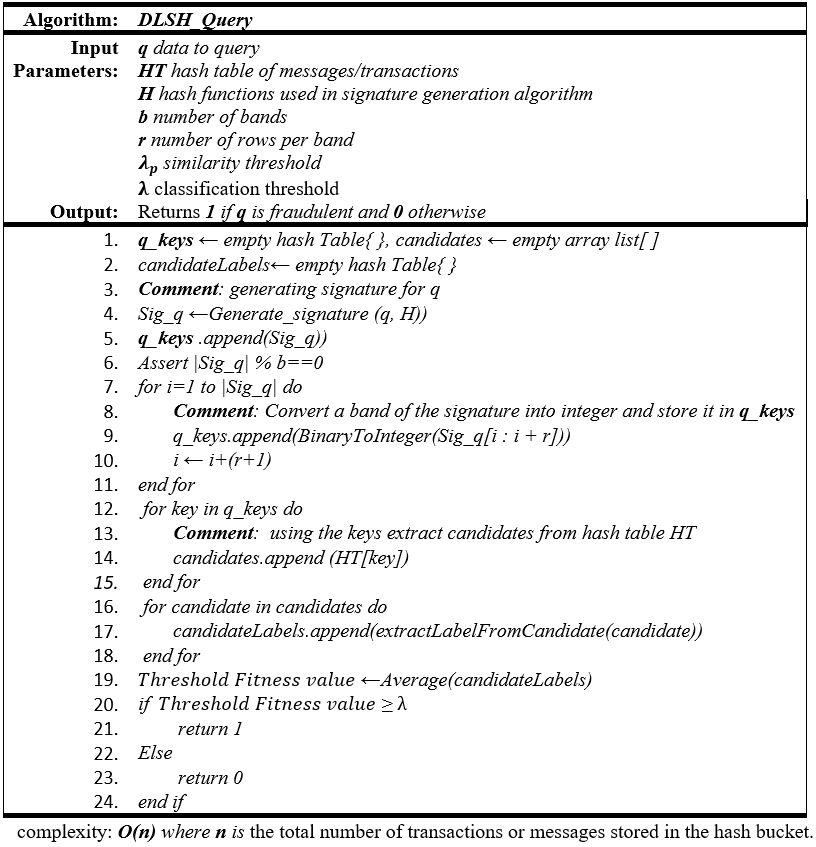
\includegraphics[width=0.7\textwidth,height=170pt]{assets/query.png}
	\end{frame}


	\begin{frame}{\raisebox{-1.9pt}{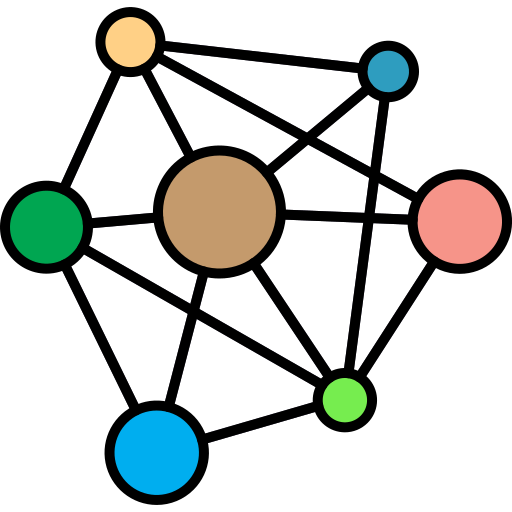
\includegraphics[width=0.5cm]{./assets/algorithm.png}} \small{Mathematical Model for Query}}
		\begin{enumerate}[1)]
			\item Let \textbf{$x$} be a sample message or transaction we want to know if its fraudulent or not
			\item Its a 2-Stage Process: Threshold Fitness Value and Threshold Fitness Extractor calculations
		\end{enumerate}
		
		\begin{columns}
			\column{0.5\textwidth}
			\small{
		\textbf{Stage 1:Threshold Fitness Value}
		\begin{center}
			\begin{enumerate}[-]
			\item $C(x)=Q(x,HT)$\\
			\item Threshold Fitness value	$ = \sum_1^n \frac{L_{cx}}{n_{cx}}$\\
		\end{enumerate}
		\end{center}
		\textbf{Stage 2:Threshold Fitness Extractor}\\
			We define a threshold value  $\lambda$ such that:\\
		\tiny{
			\begin{equation}
				Threshold Fitness Extractor =
				\begin{cases}
					1 & \text{if Threshold Fitness value $\geq \lambda$} \\
					0 & \text{otherwise}
				\end{cases}
			\end{equation}
		}
	}
			\column{0.5\textwidth}
			where:\\
			\begin{enumerate}[-]
				\item C(x) are the candidates of transaction/message x 
				\item HT is a hash table of messages or transactions 
				\item  Q is the Query function
				\item  $n_{cx}$ is the number of candidates of x. 
				\item $L_{cx}$ are the labels for C(x)  ,$L_{cx}  \in [0,1]$ 
			\end{enumerate}
		\end{columns}
 	\end{frame}
	
		\section{Results and Discussion}
		\subsection{Results and Discussion $|$ Experiment setup and Parameter configuration}
		\begin{frame}{\raisebox{-0.7pt}{
\includegraphics[width=0.5cm]{./assets/setting.png}} Experiment Setup and Parameter configuration}
		   	\begin{table}
		   	\begin{center}
		   		{\tiny
		   			%\begin{tabular}{|>{\columncolor{green}}c|c|c|c|c|c|}
		   			\begin{tabular}{|c|c|c|c|c|c|c|c|}
		   				 
		   				\hline
		   				\multicolumn{8}{|c|}{\textbf{Dynamic Locality Sensitive Hashing Experiment Parameter Configuration}}\\ 
		   				\hline
		   				\multicolumn{4}{|c|}{Mobile Money SMS} & \multicolumn{4}{|c|}{Mobile Money Transaction} \\
		   				\hline
		   				\multicolumn{2}{|c|}{Total} & \multicolumn{2}{|c|}{5,750} & \multicolumn{2}{|c|}{Total} & \multicolumn{2}{|c|}{600,000} \\
		   				\hline
		   				Test Dataset & 232 & Training Dataset & 5,175 & Test Dataset & 120,000 & Training Dataset & 480k\\
		   				\hline 
		   				\multicolumn{1}{|c|}{Similarity Threshold  \newline (${\lambda_p}$)} & \multicolumn{1}{|c|}{Band (b)} & \multicolumn{2}{|c|}{Rows (r)} & \multicolumn{1}{|c|}{Similarity Threshold \newline  (${\lambda_p}$)} &\multicolumn{1}{|c|}{Bands (b)} & \multicolumn{2}{|c|}{Rows (r)} \\
		   				\hline
		   				
		   				\multicolumn{1}{|c|}{1.0} & \multicolumn{1}{|c|}{1} & \multicolumn{2}{|c|}{512} & \multicolumn{1}{|c|}{1.0} & \multicolumn{1}{|c|}{1} & \multicolumn{2}{|c|}{1113} \\
		   				
		   				\hline 
		   				\multicolumn{1}{|c|}{0.997} & \multicolumn{1}{|c|}{2} & \multicolumn{2}{|c|}{256} & \multicolumn{1}{|c|}{0.997} & \multicolumn{1}{|c|}{3} & \multicolumn{2}{|c|}{371} \\
		   			
		   				\hline 
		   				\multicolumn{1}{|c|}{0.989} & \multicolumn{1}{|c|}{4} & \multicolumn{2}{|c|}{128} & \multicolumn{1}{|c|}{0.987} & \multicolumn{1}{|c|}{7} & \multicolumn{2}{|c|}{159} \\
		   			
		   				\hline 
		   				\multicolumn{1}{|c|}{0.968} &\multicolumn{1}{|c|}{8} & \multicolumn{2}{|c|}{64} & \multicolumn{1}{|c|}{0.944} &\multicolumn{1}{|c|}{21} & \multicolumn{2}{|c|}{53} \\
		   				
		   				\hline 
		   				\multicolumn{1}{|c|}{0.917} &\multicolumn{1}{|c|}{16} & \multicolumn{2}{|c|}{32} & \multicolumn{1}{|c|}{0.827} &\multicolumn{1}{|c|}{53} & \multicolumn{2}{|c|}{21} \\
		   				
		   				\hline 
		   				\multicolumn{1}{|c|}{0.805} &\multicolumn{1}{|c|}{32} & \multicolumn{2}{|c|}{16} & \multicolumn{1}{|c|}{0.485} &\multicolumn{1}{|c|}{159} & \multicolumn{2}{|c|}{7} \\
		   				\hline
		   				
		   				\multicolumn{1}{|c|}{0.5946} &\multicolumn{1}{|c|}{64} & \multicolumn{2}{|c|}{8} & \multicolumn{1}{|c|}{0.1391} &\multicolumn{1}{|c|}{371} & \multicolumn{2}{|c|}{3} \\
		   				\hline
		   			
		   				\multicolumn{1}{|c|}{0.2973} &\multicolumn{1}{|c|}{128} & \multicolumn{2}{|c|}{4} & \multicolumn{1}{|c|}{0.00089} &\multicolumn{1}{|c|}{1113} & \multicolumn{2}{|c|}{1} \\
		   				\hline
		   			
		   				\multicolumn{1}{|c|}{0.0625} &\multicolumn{1}{|c|}{256} & \multicolumn{2}{|c|}{2} & \multicolumn{1}{|c|}{} &\multicolumn{1}{|c|}{} & \multicolumn{2}{|c|}{} \\
		   				\hline
		   			 
		   				\multicolumn{1}{|c|}{0.00195} &\multicolumn{1}{|c|}{512} & \multicolumn{2}{|c|}{1} & \multicolumn{1}{|c|}{} &\multicolumn{1}{|c|}{} & \multicolumn{2}{|c|}{} \\
		   				\hline
		   				
		   				\multicolumn{2}{|c|}{Number of hash functions for SMS (${I_m}$)} & \multicolumn{2}{|c|}{1} & \multicolumn{2}{|c|}{} & \multicolumn{2}{|c|}{} \\
		   				\hline
		   				
		   				\multicolumn{2}{|c|}{Number of hash functions for Transaction (${I_t}$)} & \multicolumn{2}{|c|}{1} & \multicolumn{2}{|c|}{Classification Threshold (${\lambda}$)} & \multicolumn{2}{|c|}{} \\
		   				\hline
		   			\end{tabular}
		   		}
		   	\end{center}
		   	\caption{Experiment setup and parameter configuration}
		   	\label{table 1}
		   	\end{table}
		\end{frame}
		
		
		
			\begin{frame}{Review of State of the art Mobile Money Prediction and detection Systems}
				\small{Mobile Money SMS fraud detection and prediction}
			\begin{table}
				\begin{center}
					{\tiny
						%\begin{tabular}{|>{\columncolor{green}}c|c|c|c|c|c|}
						\begin{tabular}{ | m{0.2cm} | m{1 cm} | m{1 cm} | m{1 cm} | m{1 cm} | m{1 cm} | m{1 cm} | m{1 cm} |m{1 cm} | m{1 cm} |}  
							\hline
							ID &Message (M) & Encoded M & signature M & $\lambda_p$ & Bucket ID(s) & Candidate ID(s) & Threshold fitness value & Fitness Extraction & Label \\
							\hline
						
						\end{tabular}
					}
				\end{center}
				\caption{Review of State of the Art Technique}
				\label{table 1}
			\end{table}
		
		\small{Mobile Money Transaction fraud detection and prediction}
			\begin{table}
			\begin{center}
				{\tiny
					%\begin{tabular}{|>{\columncolor{green}}c|c|c|c|c|c|}
					\begin{tabular}{ | m{0.2cm} | m{1 cm} | m{1 cm} | m{1 cm} | m{1 cm} | m{1 cm} | m{1 cm} | m{1 cm} |m{1 cm} | m{1 cm} |}  
						\hline
						ID &Message (M) & Encoded M & signature M & $\lambda_p$ & Bucket ID(s) & Candidate ID(s) & Threshold fitness value & Fitness Extraction & Label \\
						\hline
						
					\end{tabular}
				}
			\end{center}
			\caption{Review of State of the Art Technique}
			\label{table 1}
		\end{table}
		\end{frame}
		
		
		
			\subsection{Results and Discussion $|$ Efficiency}
			\begin{frame}{$|$\raisebox{-0.7pt}{
\includegraphics[width=0.5cm]{./assets/setting.png}} \footnotesize{RQ1: How can we use a novel dynamic locality sensitive hashing techniques to efficiently detect and predict         mobile money SMS fraud?}}
				%somecontent here
				\begin{columns}
					\column{0.5\textwidth}
					
						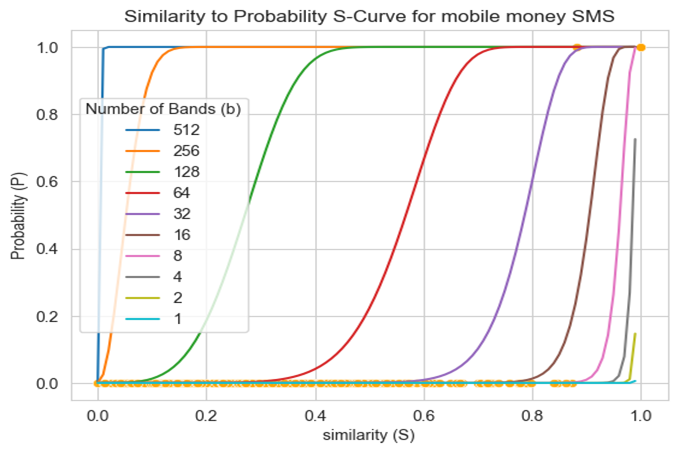
\includegraphics[width=225pt, height=150pt]{assets/smseff.png}
						\centering{\textbf{575 Mobile Money Messages}}
						
					
					\column{0.5\textwidth}
						
						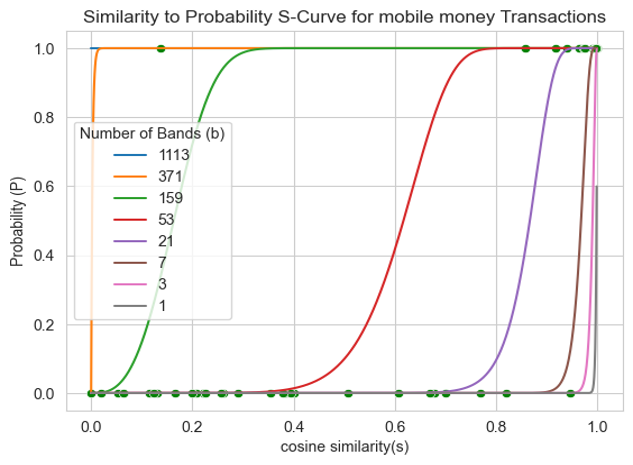
\includegraphics[width=225pt, height=150pt]{assets/transeff.png}
						\centering{\textbf{1200 Mobile Money transactions}}
					
				\end{columns}
			\end{frame}
		

		
		\subsection{Results and Discussion $|$ Efficiency}
		\begin{frame}{$|$ {$|$ \footnotesize{RQ2: How can we use a novel dynamic locality sensitive hashing techniques to Rapidly detect and predict         mobile money SMS fraud?}}}
			%somecontent here
				\begin{columns}
				\column{0.5\textwidth}
	
				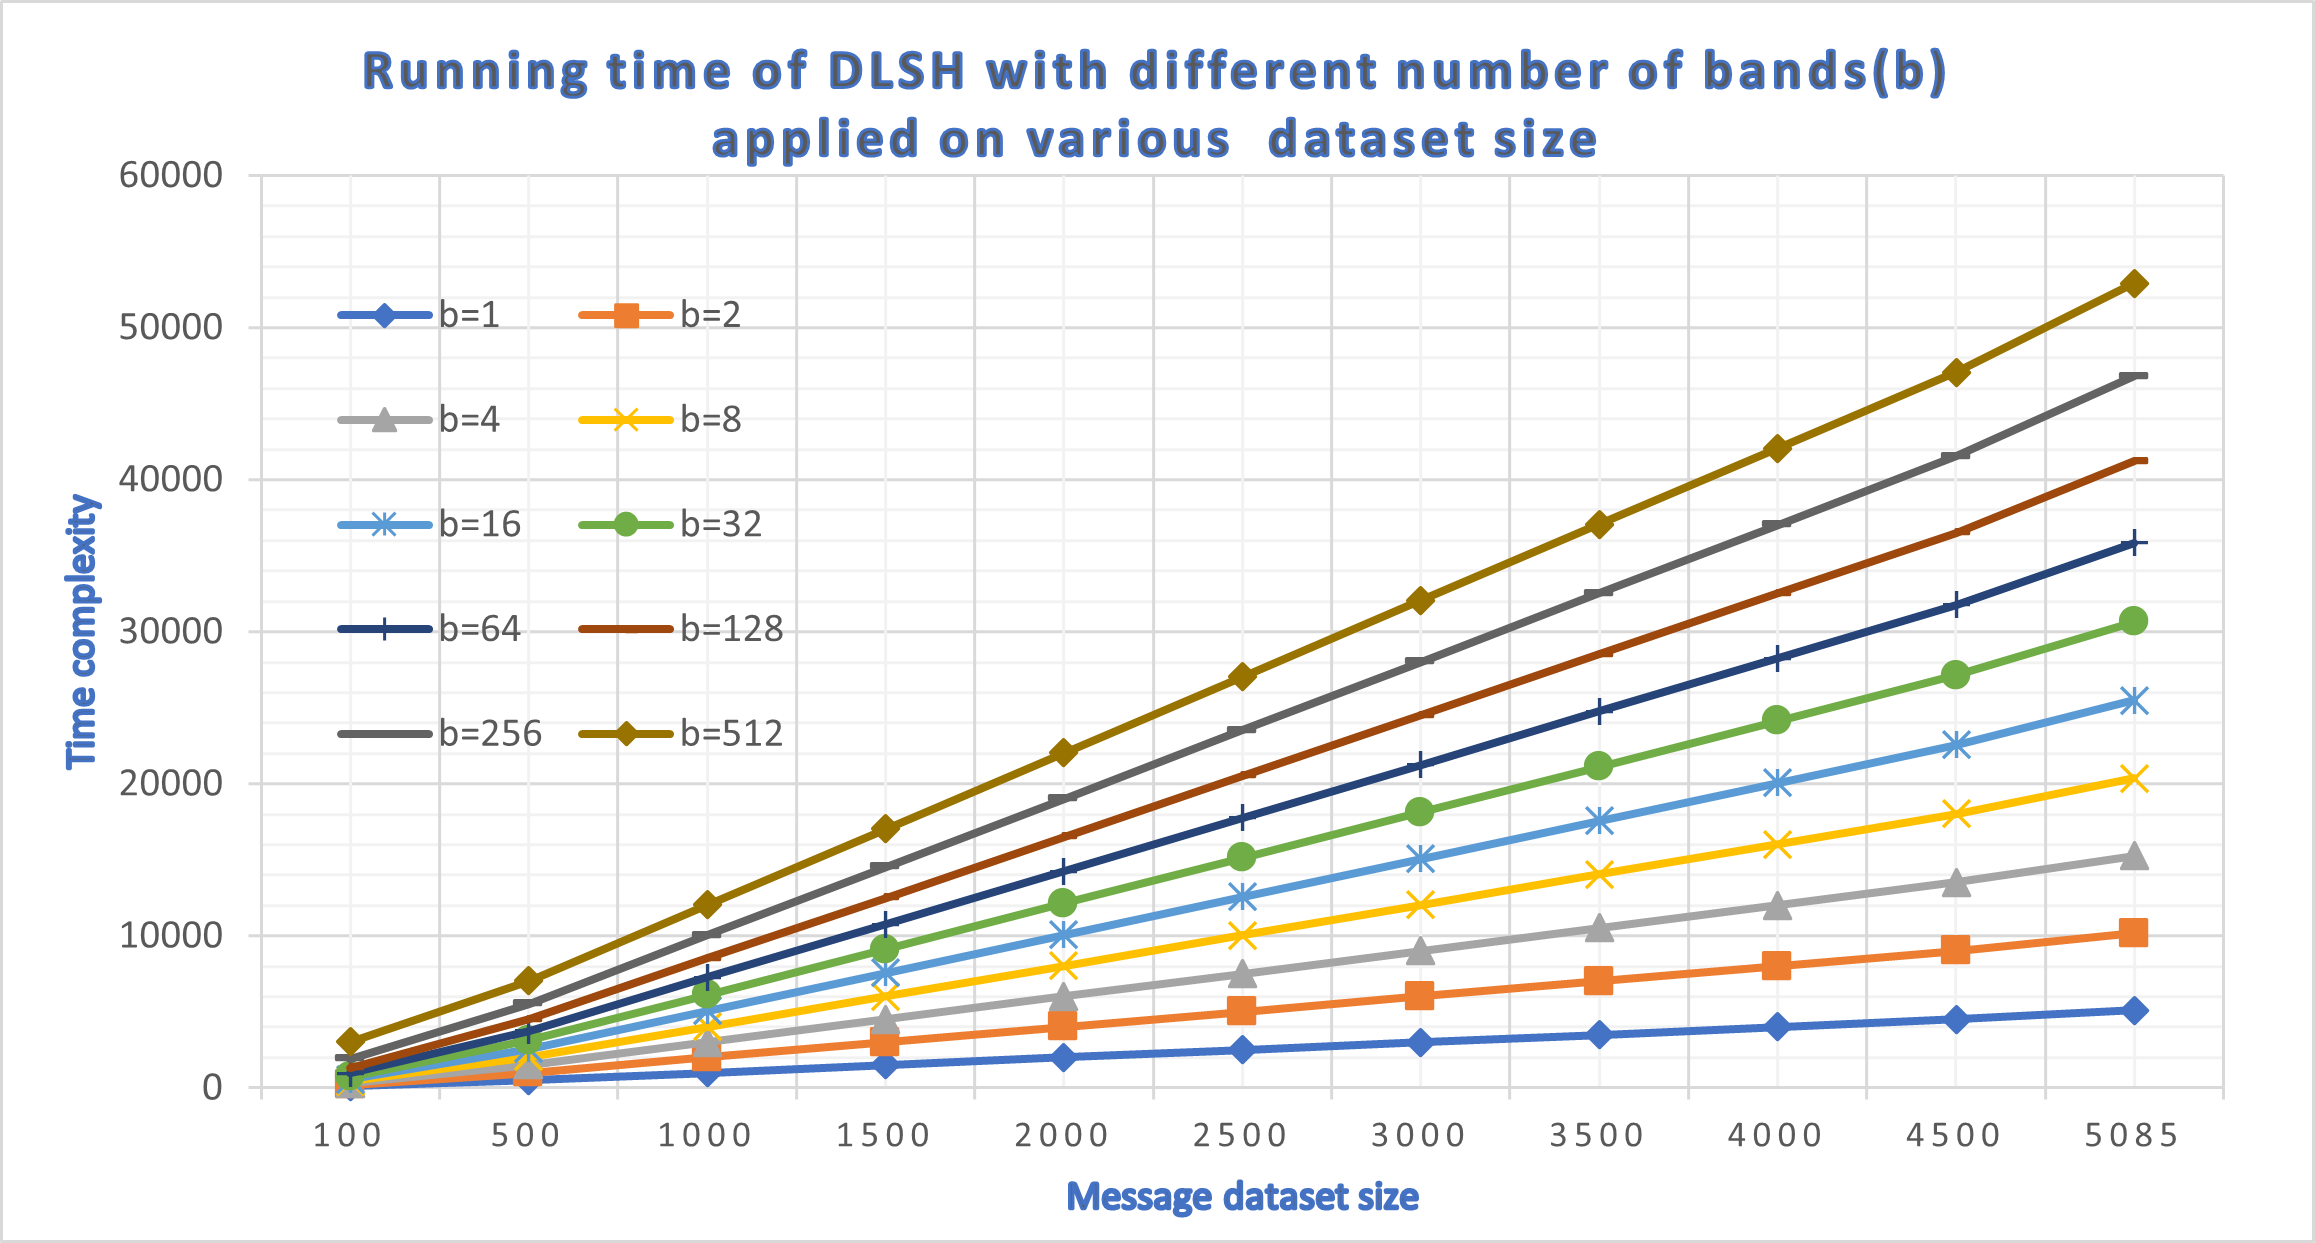
\includegraphics[width=225pt, height=75pt]{assets/smseff1.png}
				
				
				
				\column{0.5\textwidth}
				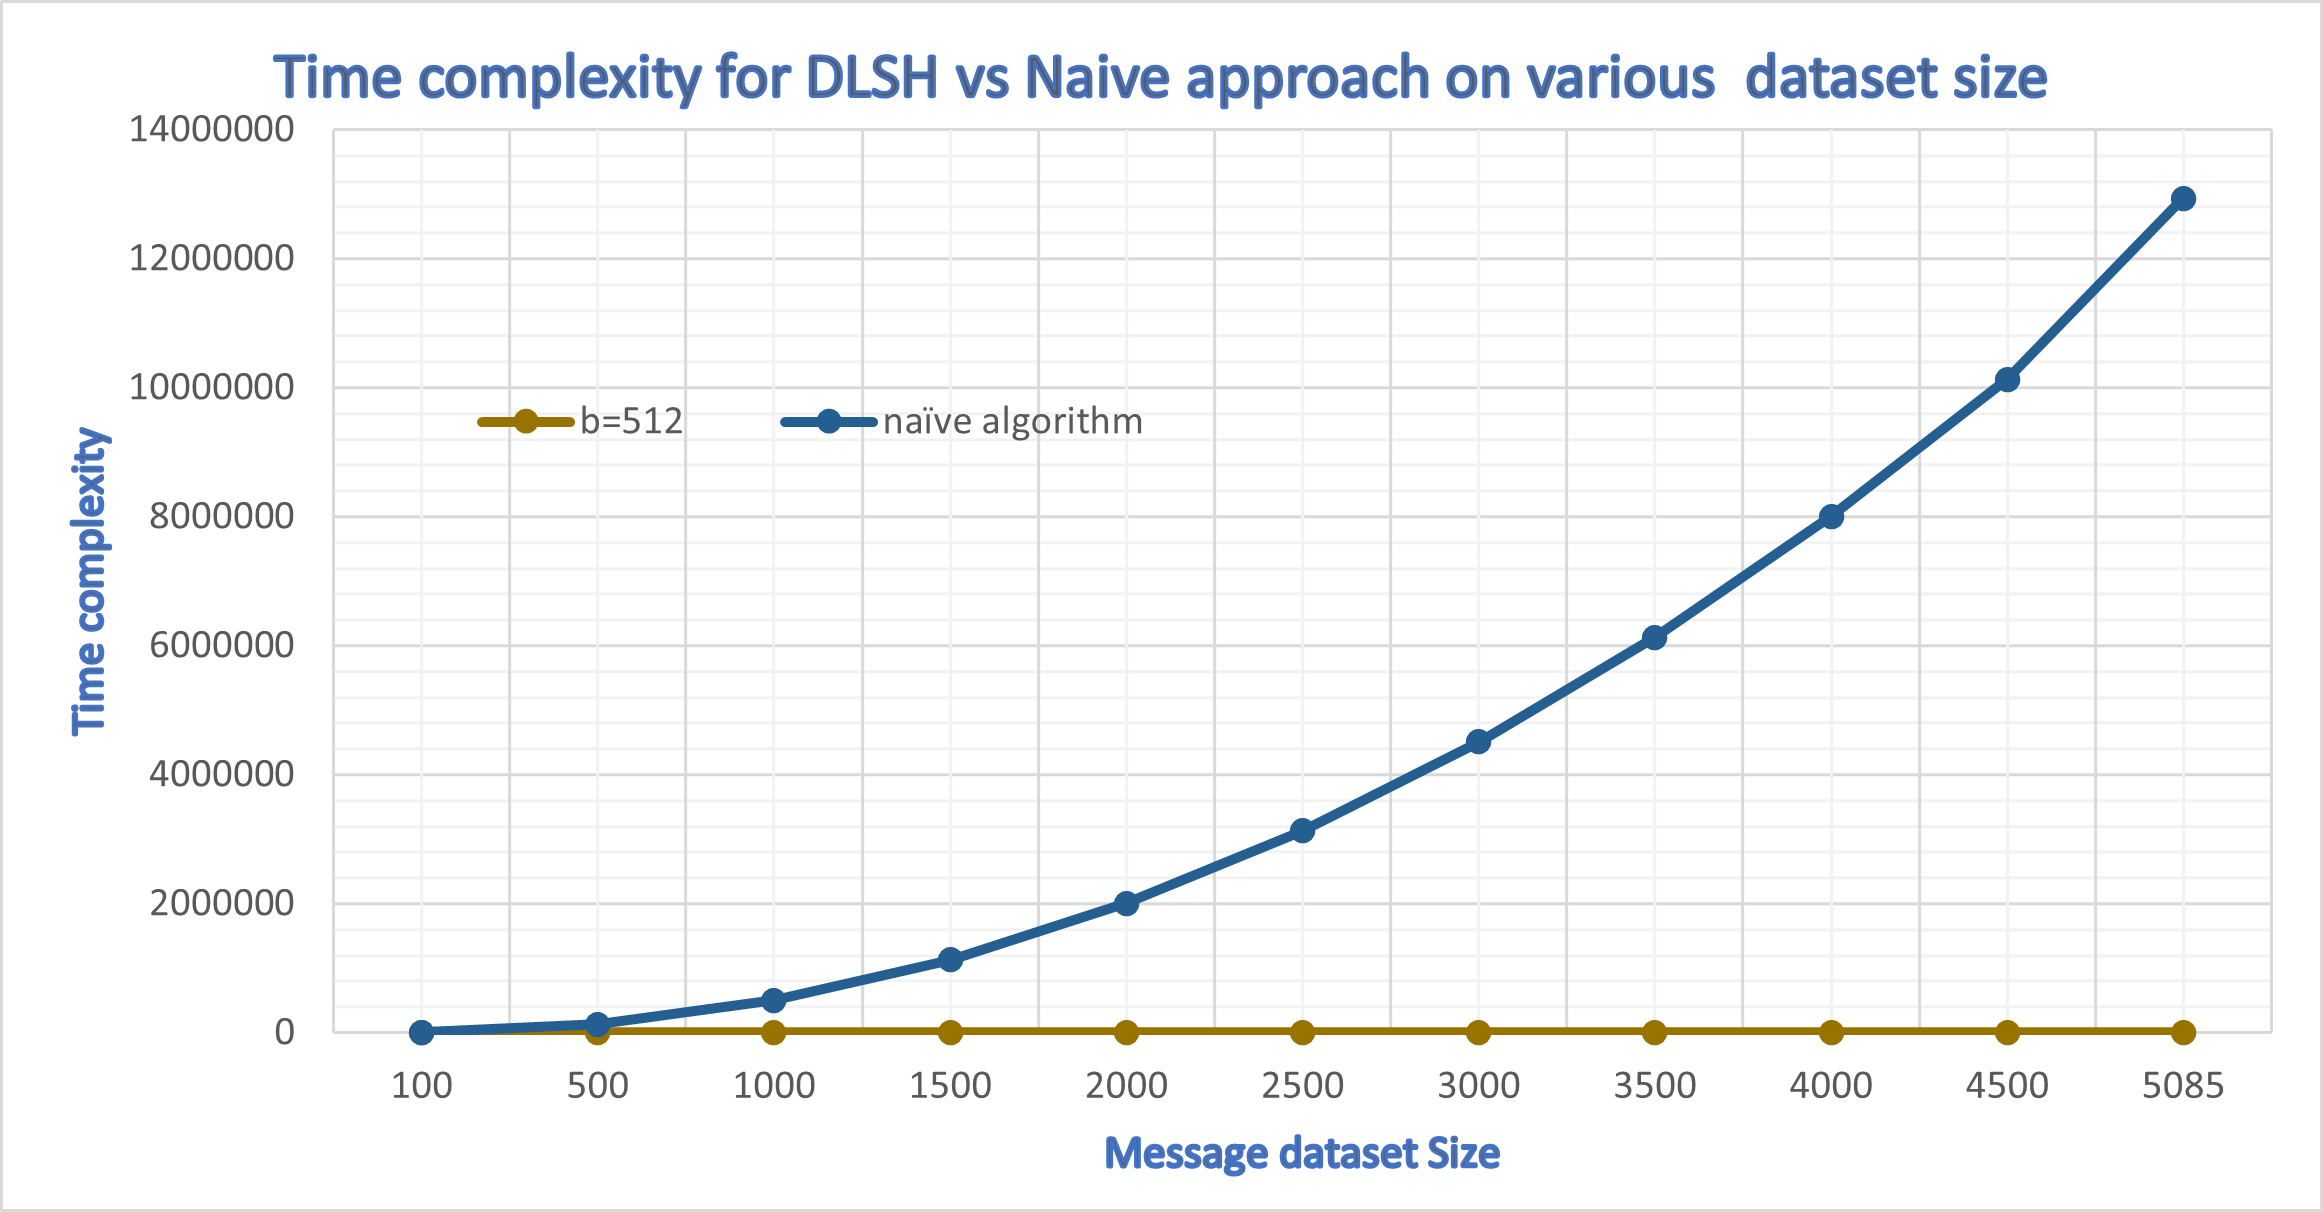
\includegraphics[width=225pt, height=75pt]{assets/naivesmseff2.png}
				
				
			\end{columns}
			\begin{columns}
			\column{0.5\textwidth}
			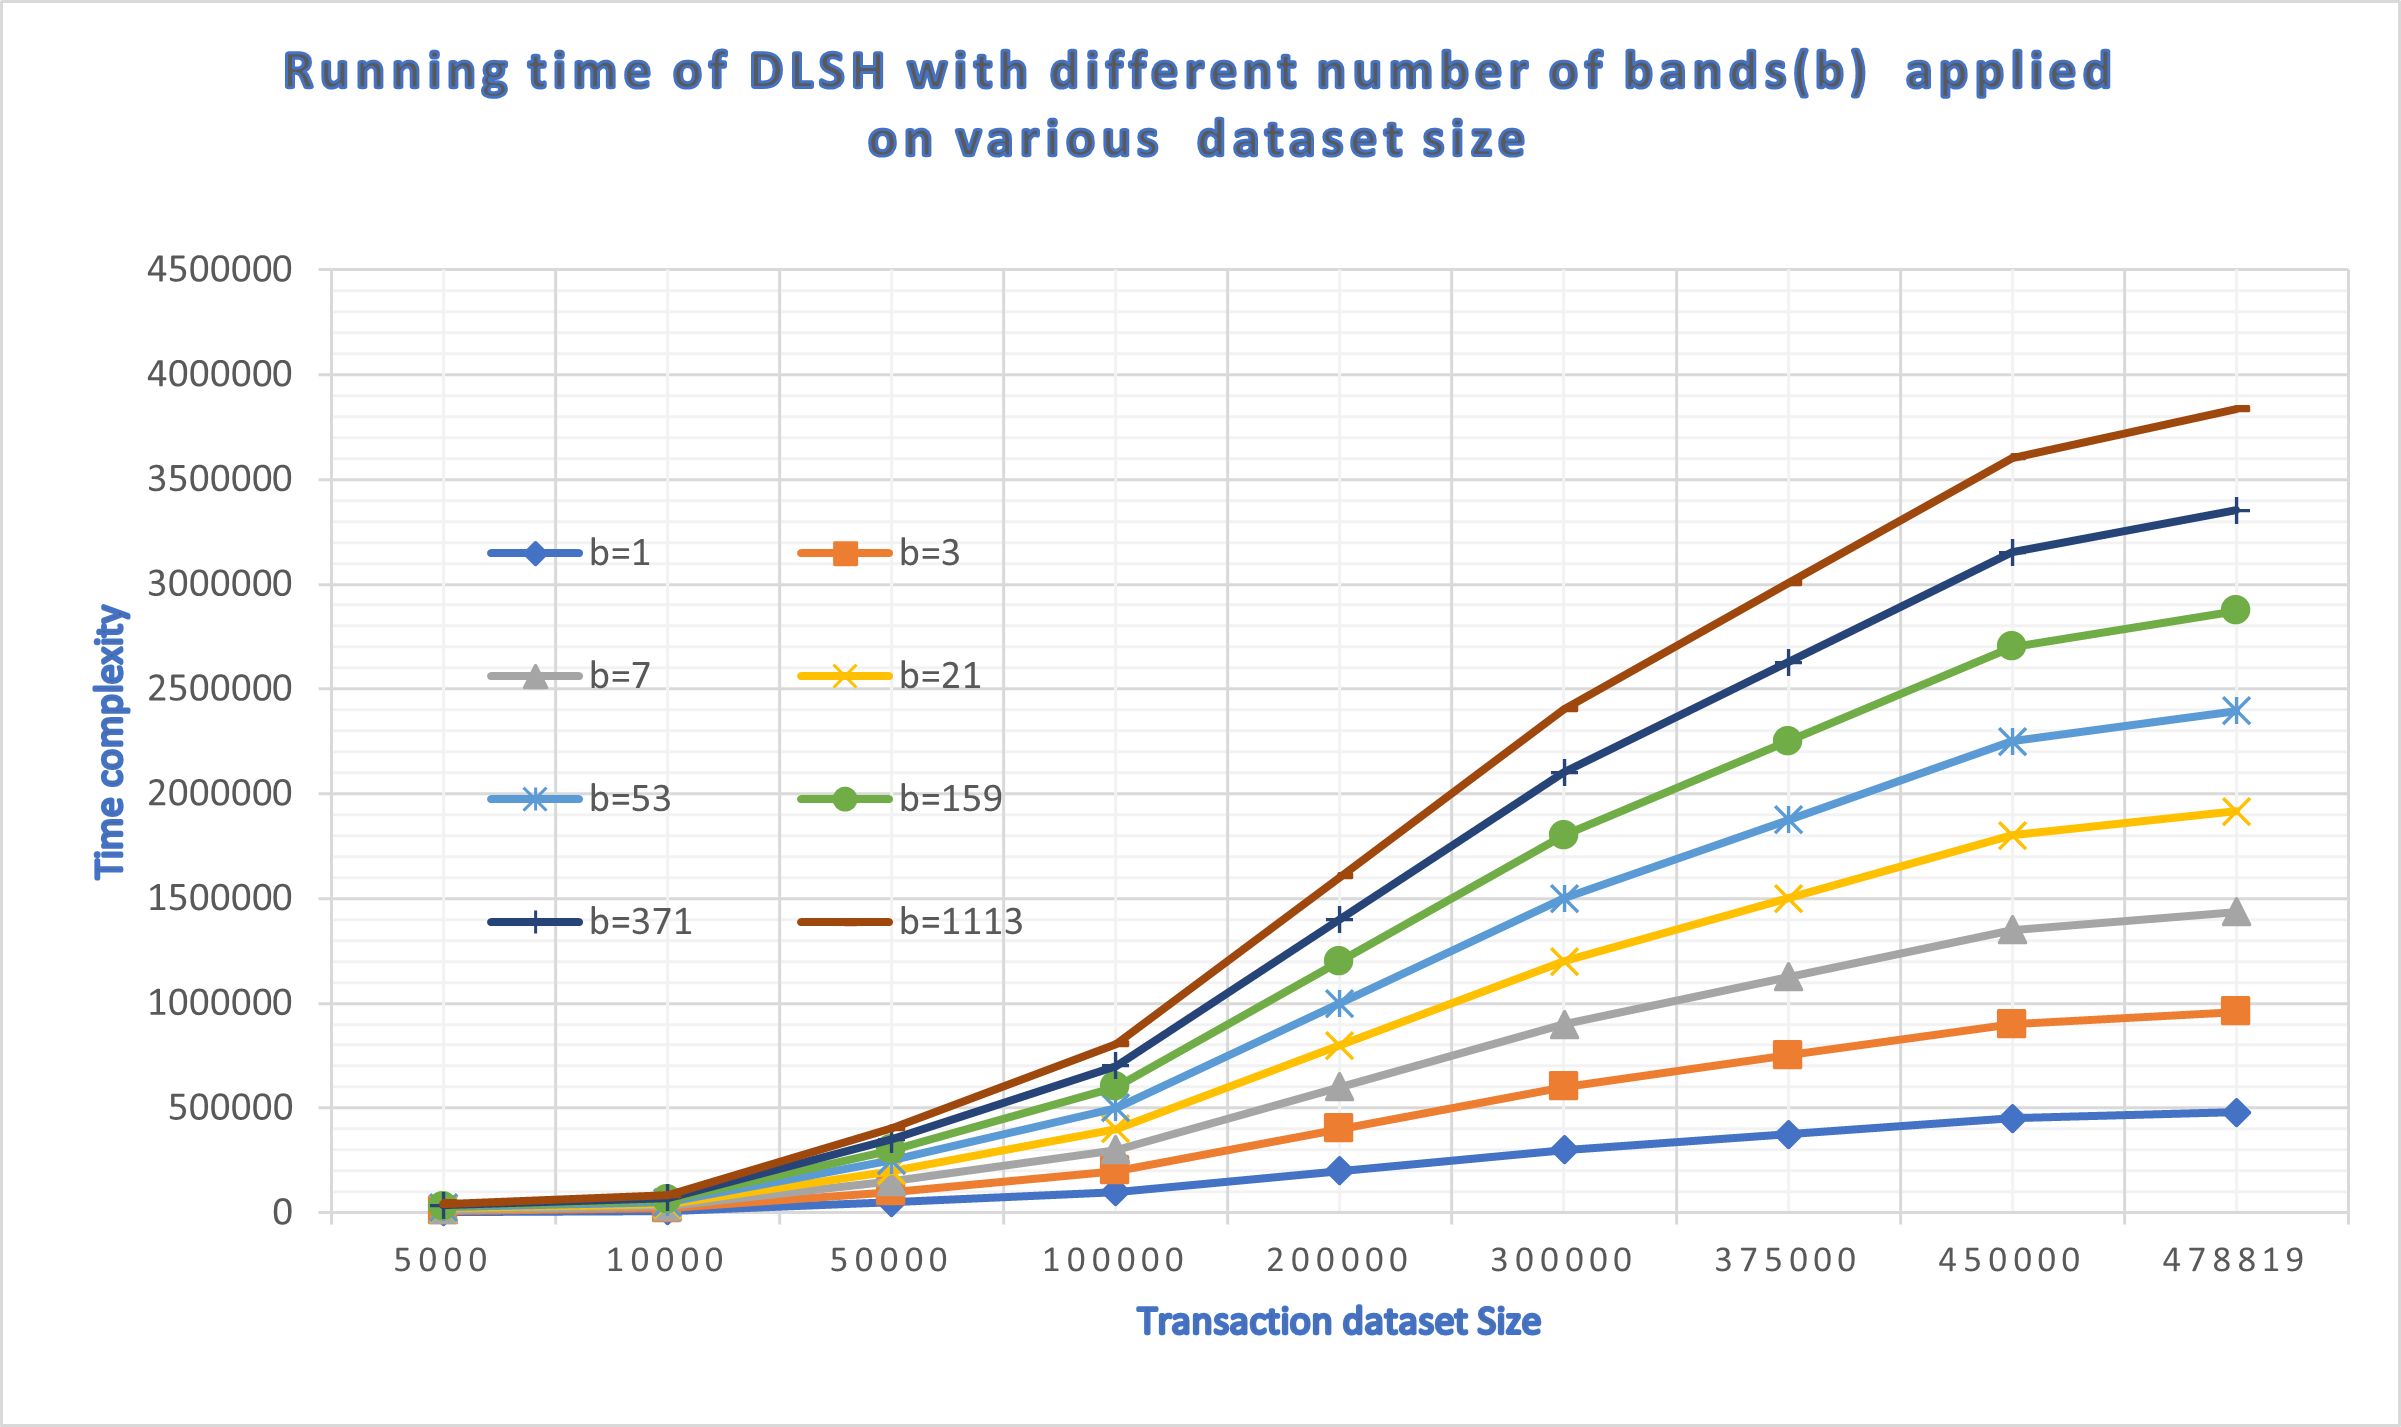
\includegraphics[width=225pt, height=75pt]{assets/transeff1.png}

			
			
			\column{0.5\textwidth}
			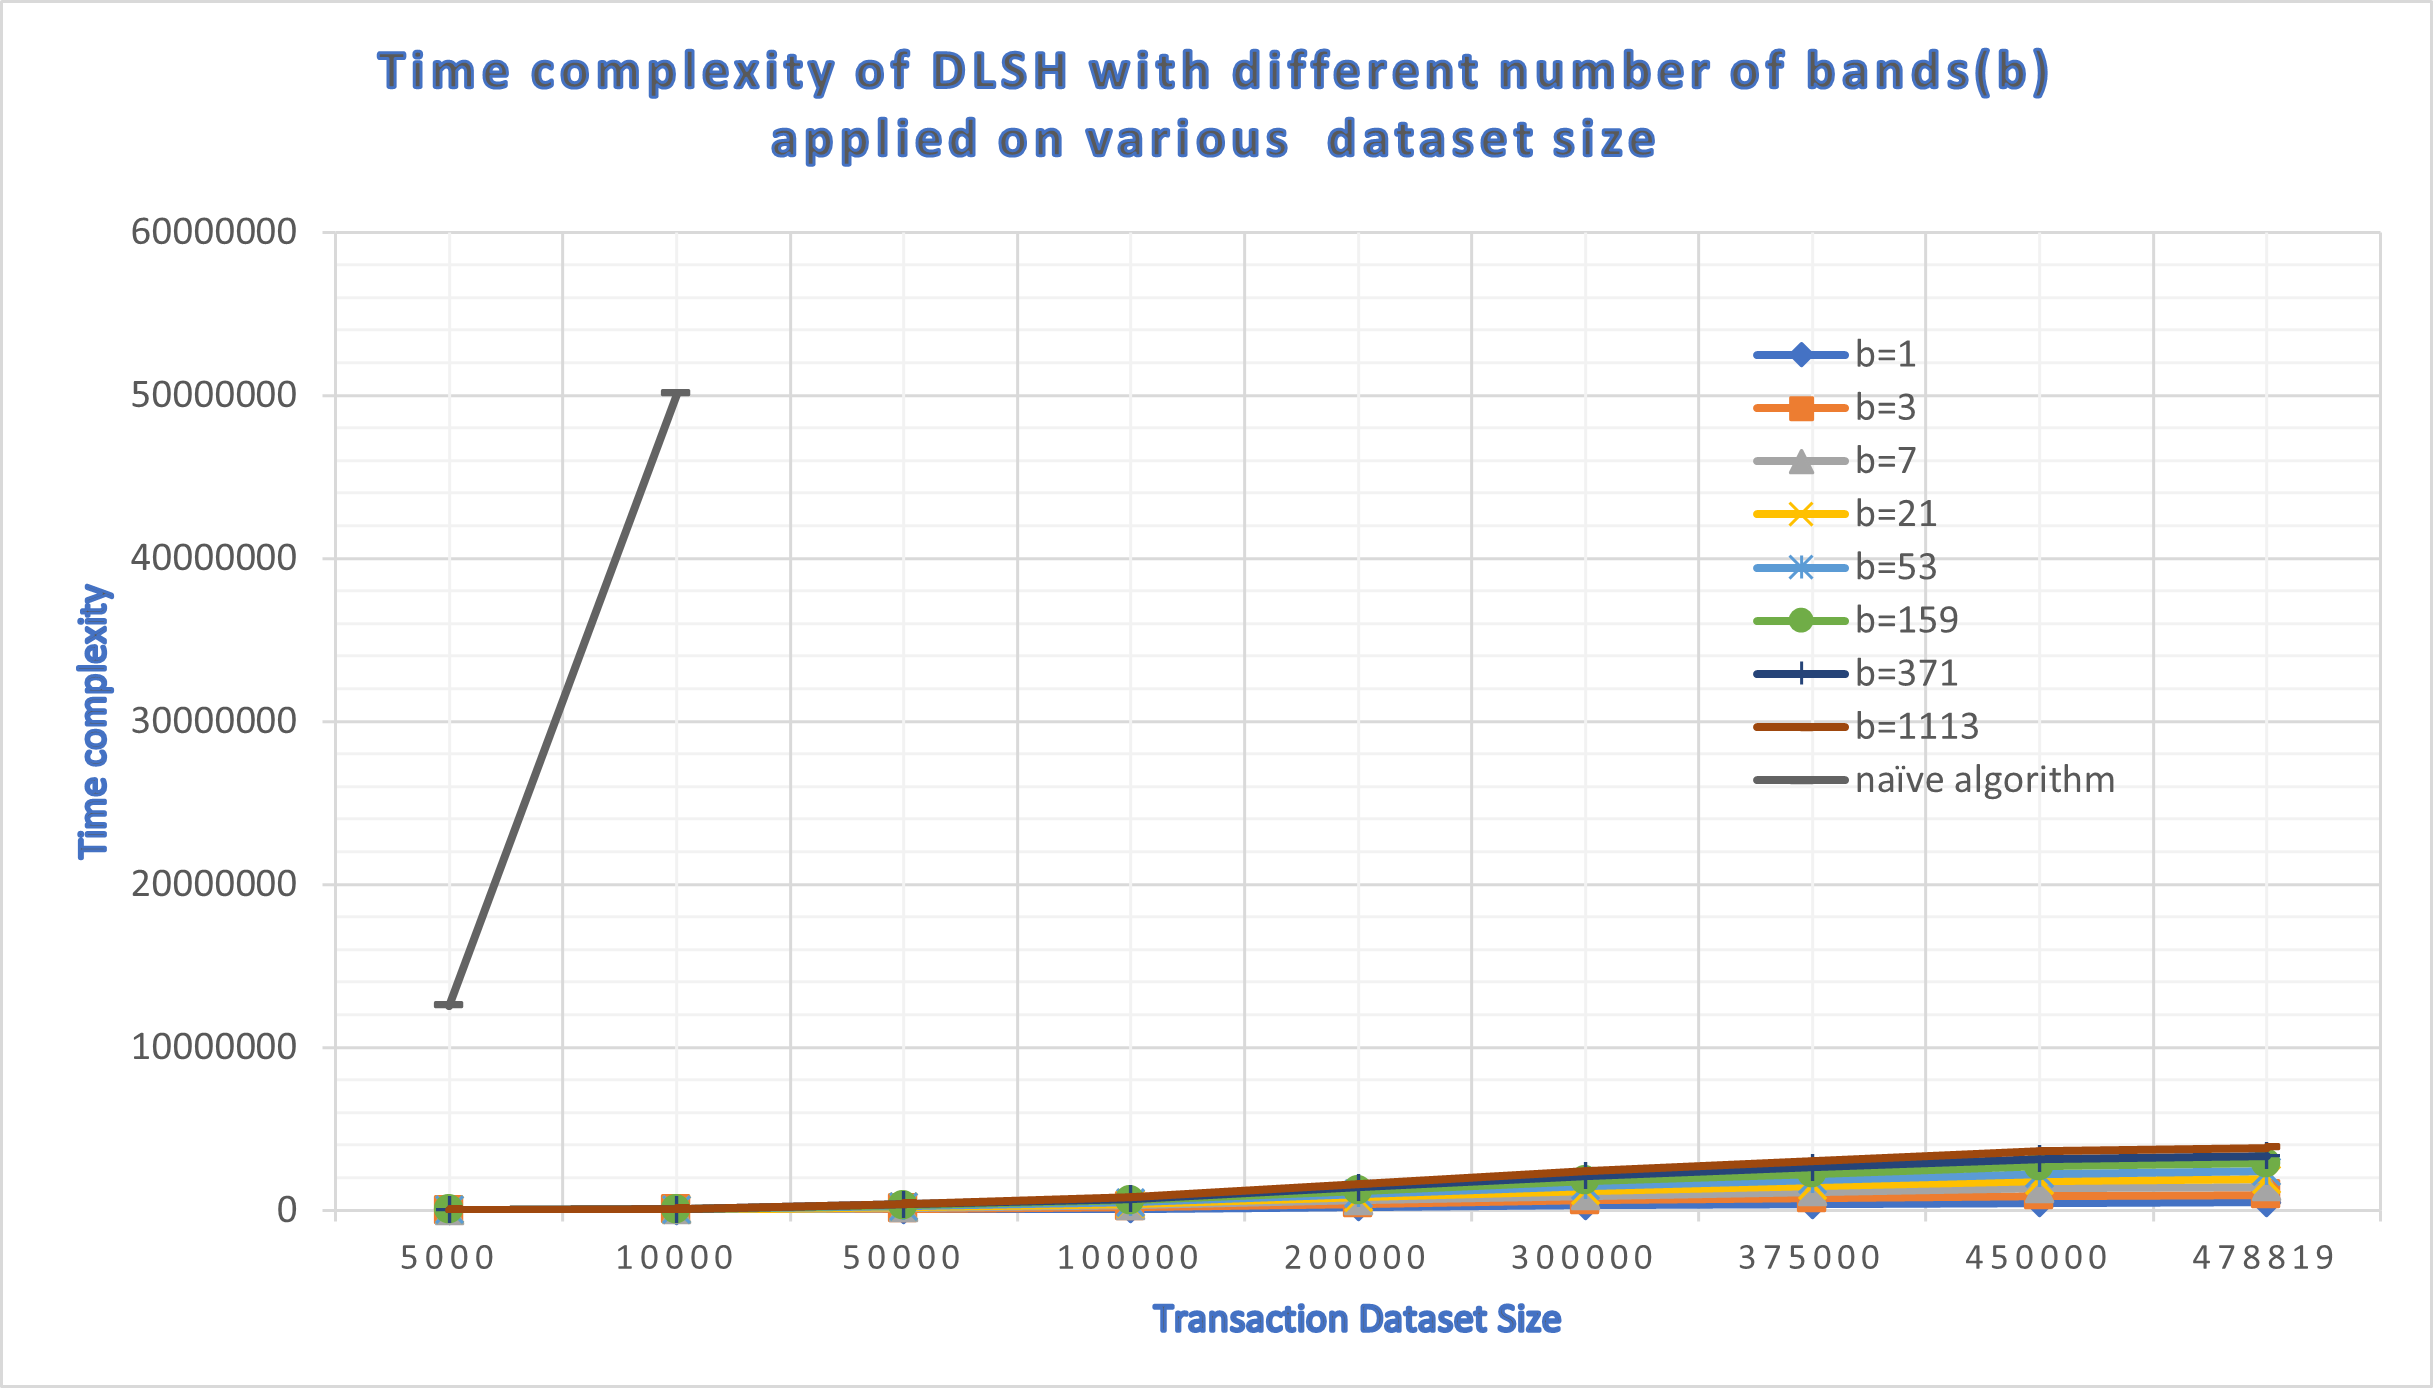
\includegraphics[width=225pt, height=75pt]{assets/transnaiveeff.png}
		
		\end{columns}
			
			
		\end{frame}
	
	
		\subsection{Results and Discussion $|$ Efficiency}
		\begin{frame}{DLSH Comparison with State of the Art}
				%somecontent here
			\begin{table}
				\begin{center}
					{\tiny
						%\begin{tabular}{|>{\columncolor{green}}c|c|c|c|c|c|}
							 \begin{tabular}{ |>{\columncolor{green}} m{3 cm} | m{2.5 cm} | m{1.5 cm} | m{1 cm} | m{2 cm} | m{1.5 cm} |}  
							\hline
							\rowcolor{orange}
							Approach & Efficiency & Speed & Scalability & Detection and prediction ability & Computational cost \\
							\hline
							
							\textbf{Dynamic Locality Sensitive hashing  (our approach)}
							& -	SMS: 98.6 \% \newline
							-Transaction: 99\%
							 & Very Fast
							& YES &  - SMS \newline -Transaction & Low \\
							\hline
							
							\textbf{Case based reasoning [8]}
							& 98\% prediction efficiency\newline & Fast & NO & Transaction& Very High \\
							\hline
							
							\textbf{Cross-case analysis Approach [7]}
							& - Support Vector Machine: 99.91\% \newline
							- Naïve Bayes algorithm: 99.65\% \newline
							- Gradient boosted Decision tree: 89.9\% \newline
							 & Fast & YES & Transaction& High \\
							\hline
							
						
							
							\textbf{Mobile money SMS fraud detection [23]}
							& 99.82$\%$ & Fast& YES & SMS& High\\
							
							\hline
							
						\end{tabular}
					}
				\end{center}
			\caption{DLSH comparison with State of the Art}
			\label{table 1}
			\end{table}
			
		\end{frame}
		
		
	\subsection{Results and Discussion $|$ Efficiency}
		\begin{frame}{Tools and Technologies used}
			\begin{columns}
				
				\column{0.5\textwidth}
					\begin{block}{Integrated Development Environment}
						\begin{itemize}
							\item Data spell
							\item Visual studio code
						\end{itemize}
					\end{block}
					\begin{block}{Platforms}
					
					\begin{itemize}
						\item Kaggle
						\item Github
						
					\end{itemize}
				\end{block}
				
					\column{0.5\textwidth}

					\begin{block}{Libraries}
						\begin{enumerate}[(1)]
							\item Numpy
							\item Pandas
							\item Sci-Kit Learn
							\item Google Universal Sentence Encoder
							\item Seaborn
							\item Matplotlip
							\item Xgboost
						\end{enumerate}
					\end{block}
				
				
				
			\end{columns}
		\end{frame}
	
	
	\section{Conclusion}
		\subsection{Contributions and Difficulties encountered}
		\begin{frame}
			%somecontent here
			\begin{block}{Contribution}
				\begin{enumerate}[i)]
					\item We Introduced a Novel Approach to Mobile money fraud detection and prediction using Dynamic Locality sensitive Hashing
					
					
					\item Approach could tackle  both SMS and Transaction Fraud
					
					
					\item Approach was efficient on SMS (98.6$\%$) and Transaction(99$\%$) datasets
					
					
					
				\end{enumerate}
				
			\end{block}
	
		
			\begin{block}{Difficulties}
				\begin{enumerate}
					\item Difficulty in obtaining real world company data for the research work. 
					
					\item Difficulty in gaining access to the servers of a real mobile money service provider in order to test the approach
			\end{enumerate}
			\end{block}
		\end{frame}
	
		\subsection{Recommendations for future studies}
		\begin{frame}
			\begin{block}{Recommendations for future studies}
				\begin{itemize}
					\item Explore means of apply DLSH to taggling Mobile fraud related to fraudulent calls
					
					\item Extend DLSH to tackle process related fraud such as money laundry within the mobile money sector
					
					\item Implement the proposed architecture on a distributed computing model such as Map-Reduce which will drastically increase the speed 
					
			
					\item Extend DLSH to related financial domains such as bank transactions.
					\item Adapt DLSH to handle Mobile Money Fraud involving SIM Swap
					
				\end{itemize}
			\end{block}
		\end{frame}
	
	
			
			\subsection{References}
			\begin{frame}
			\begin{block}{References}
				\begin{itemize}
					\small
					
					\item	$[6]$	R. Rieke, M. Zhdanova, J. Repp, R. Giot, and C. Gaber, “Fraud Detection in Mobile Payments Utilizing Process Behavior Analysis,” 2013. [Online]. Available: https://hal.archives-ouvertes.fr/hal-00841002
					
					\item 	$[7]$	F. E. Botchey, Z. Qin, and K. Hughes-Lartey, “Mobile money fraud prediction-A cross-case analysis on the efficiency of support vector machines, gradient boosted decision trees, and Naïve Bayes algorithms,” Information (Switzerland), vol. 11, no. 8, Aug. 2020, doi: 10.3390/INFO11080383.
					
					\item	$[8]$	A. Adedoyin, S. Kapetanakis, G. Samakovitis, and M. Petridis, “Predicting fraud in mobile money transfer using case-based reasoning,” Lecture Notes in Computer Science (including subseries Lecture Notes in Artificial Intelligence and Lecture Notes in Bioinformatics), vol. 10630 LNAI, pp. 325–337, 2017, doi: 10.1007/978-3-319-71078-5$\_$28
					
					\item	$[23]$	J. Nkoy and A. Mohammed, “Mobile Money SMS Fraud Detection,” Stanford CS 229 Final Project Report.
					transactions. (2021)
					
				\end{itemize}
			\end{block}
		\end{frame}
	
	\subsection{Gratitude and submission for Questioning}
	\begin{frame}
		\begin{columns}
		
			\column{0.7\textwidth}
			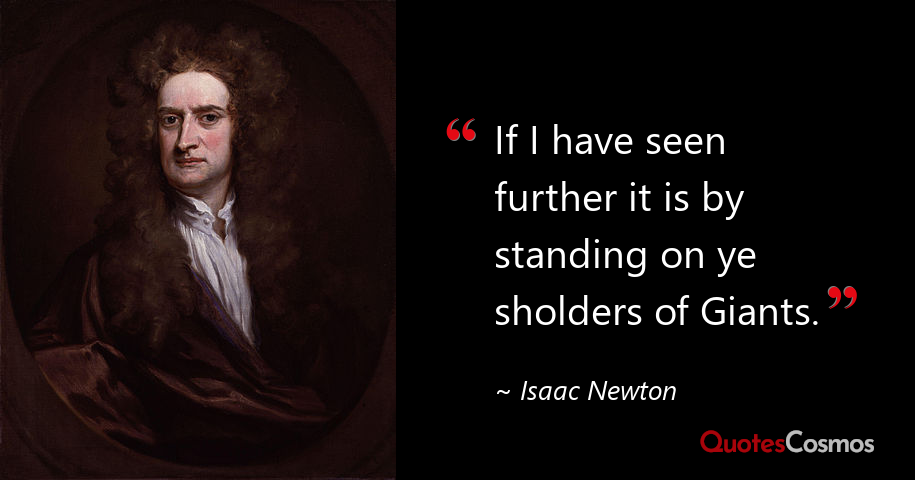
\includegraphics[width=\textwidth,  height=150pt]{./assets/Isaac.png}
			\column{0.3\textwidth}
			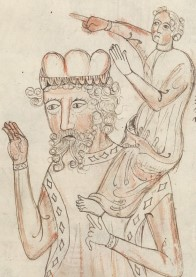
\includegraphics[width=\textwidth,  height=150pt]{./assets/stand.jpg}
		\end{columns}
	
	\begin{columns}
		\column{\textwidth}
		\\
			\centering \huge{\underline{Thanks for Your Kind Attention}}
	\end{columns}
	\end{frame}
\end{document}
